\section{Boosted Decision Tree Technique}
\label{sec:BDT}
We use the Boosted Decision Tree (BDT) Multivariate analysis technique to 
distinguish between the signal and background. This method 
combines several variables and their correlation information to construct a single discriminator variable that has a better separation power. 
The BDT technique method is implemented in the TMVA framework \cite{Therhaag:2010zz}, which is part of the ROOT package. As we will 
demonstrate in this section, this method provides a considerable saperation between signal and background shape.
The BDT technique is divided in two sections: the first one, called training, 
where the discriminator is constructed, and the second part, called classification, where this variable is evaluated in data and background.

\subsection{BDT Variables}
For a better performance of the BDT technique, well modeled variables are required. We look at 
several variables including individual and global kinematics variables, and some others based on 
angular correlations. To choose the best ones for this analysis, we look at the agreement, after 
selection, between data and background, given by the value of the Kolmogorov-Smirnov (KS) Test,  
and the performance of the BDT training. 

\subsubsection{Definition and Selection of Event Variables}
The training variables that we use in the BDT analysis can be divided into three Tables.~\ref{tab:objkin}-~\ref{tab:recoangu}:

\begin{table}[h!]
\small
\begin{center}
\begin{tabular}{|c|c|}
\hline
Variable & Definition\\ \hline
lepton $p_{T}$  & Lepton $p_{T}$ \\ \hline
lepton $\eta$ & Lepton $\eta$ \\ \hline
Tagjet1 $p_{T}$ & Leading jet $p_{T}$ \\ \hline
Tagjet1 $\eta$ & Leading jet $\eta$ \\ \hline
Tagjet2 $p_{T}$ & Second leading jet $p_{T}$ \\ \hline
Tagjet2 $\eta$ & Second leading jet $\eta$ \\ \hline
\end{tabular}
\caption{Object Kinematic Variables}
\label{tab:objkin}
\end{center}
\end{table}

%Object Angular Variables:
\begin{table}[h!]
\small
\begin{center}
\begin{tabular}{|c|c|}
\hline
Variable & Definition\\ \hline
$\Delta \eta (j1,j2)$ & $\Delta \eta$ of two tag jet\\ \hline
$\sum \eta (j1,j2)$ & Sum of two tag jet $\eta$\\ \hline
$\Delta \phi (j1,j2)$ & $\Delta \phi$ of two tag jet \\\hline
$\Delta \eta (W,j1)$ & $\Delta \eta$ of leptonic W and leading jet \\\hline
$\Delta \eta (W,j2)$ & $\Delta \eta$ of leptonic W and second leading jet \\\hline
$\Delta \phi (W,j1)$ & $\Delta \phi$ of leptonic W and leading jet \\\hline
$\Delta \phi (W,j2)$ & $\Delta \phi$ of leptonic W and second leading jet \\\hline
Zeppenfeld variable & $|y_{W} -(y_{jet1} + y_{jet2})/2.0|$\\ \hline
\end{tabular}
\caption{Object Angular Variables}
\label{tab:objang}
\end{center}
\end{table}
      
%Composite and Reconstructed Object Angular and Kinematic Variables:
%\caption{Composite and Reconstructed Object Angular and Kinematic Variables}
\begin{table}[h!]
\small
\begin{center}
\begin{tabular}{|c|c|}
\hline
Variable & Definition\\ \hline
W $p_{T}$ & Leptonic W $p_{T}$\\ \hline
W $\eta$ & Leptonic W $\eta$\\ \hline
$m_{j1,j2}$ & Tagjet pair invariant mass $m_{jj}$\\ \hline
\end{tabular}
\caption{Composite and Reconstructed Object Angular and Kinematic Variables}
\label{tab:recoangu}
\end{center}
\end{table}

We first reconstruct the leptonic W candidate. We compute the $p_z$ component of the neutrino to fully reconstruct the leptonic W four momentum.
We assume that the lepton and the MET arise from a $W$ (mass=80.4 GeV) parent. This gives a quadratic equation for $p_z$, solvable up to a two-fold ambiguity. In the case we have complex solutions, we take the real part as the solution and recalculate the $pT$ of the neutrino to remove the imaginary part (see Appendix~\ref{App:Pzneutrino}). In the case of two real roots, the neutrino $p_{z}$ solution which is closer to lepton $p_{z}$ is selected.

The training variables distribution are shown From Figs.~\ref{fig:lepw_pt} to ~\ref{fig:deltaphiwj2} in the control region. Some variables distributuin have already been shown before and they will not be shown here. 
%We loop two neutrino candidates and all the jets to select the combination that gives the nearest mass to that of the top quark ( 172.5 ~GeV ).

%Figure~\ref{fig:lepwmass} shows the invariant mass of the leptonic $W$, which is obtained using the solution found for the neutrino momentum  for the \muons and the 
%\electrons samples. The events with mass above and below the $W$ mass are due 
%to solutions with complex roots that arise from uncertainties in the measurement of the missing transverse momentum.
%The invariant mass of the reconstructed leptonic top candidates are shown in Figure~\ref{fig:leptopmass}.
%This distribution peaks at the expected top mass. The large tail is due to the MET resolution.

\begin{figure}[ht]
\centerline{
   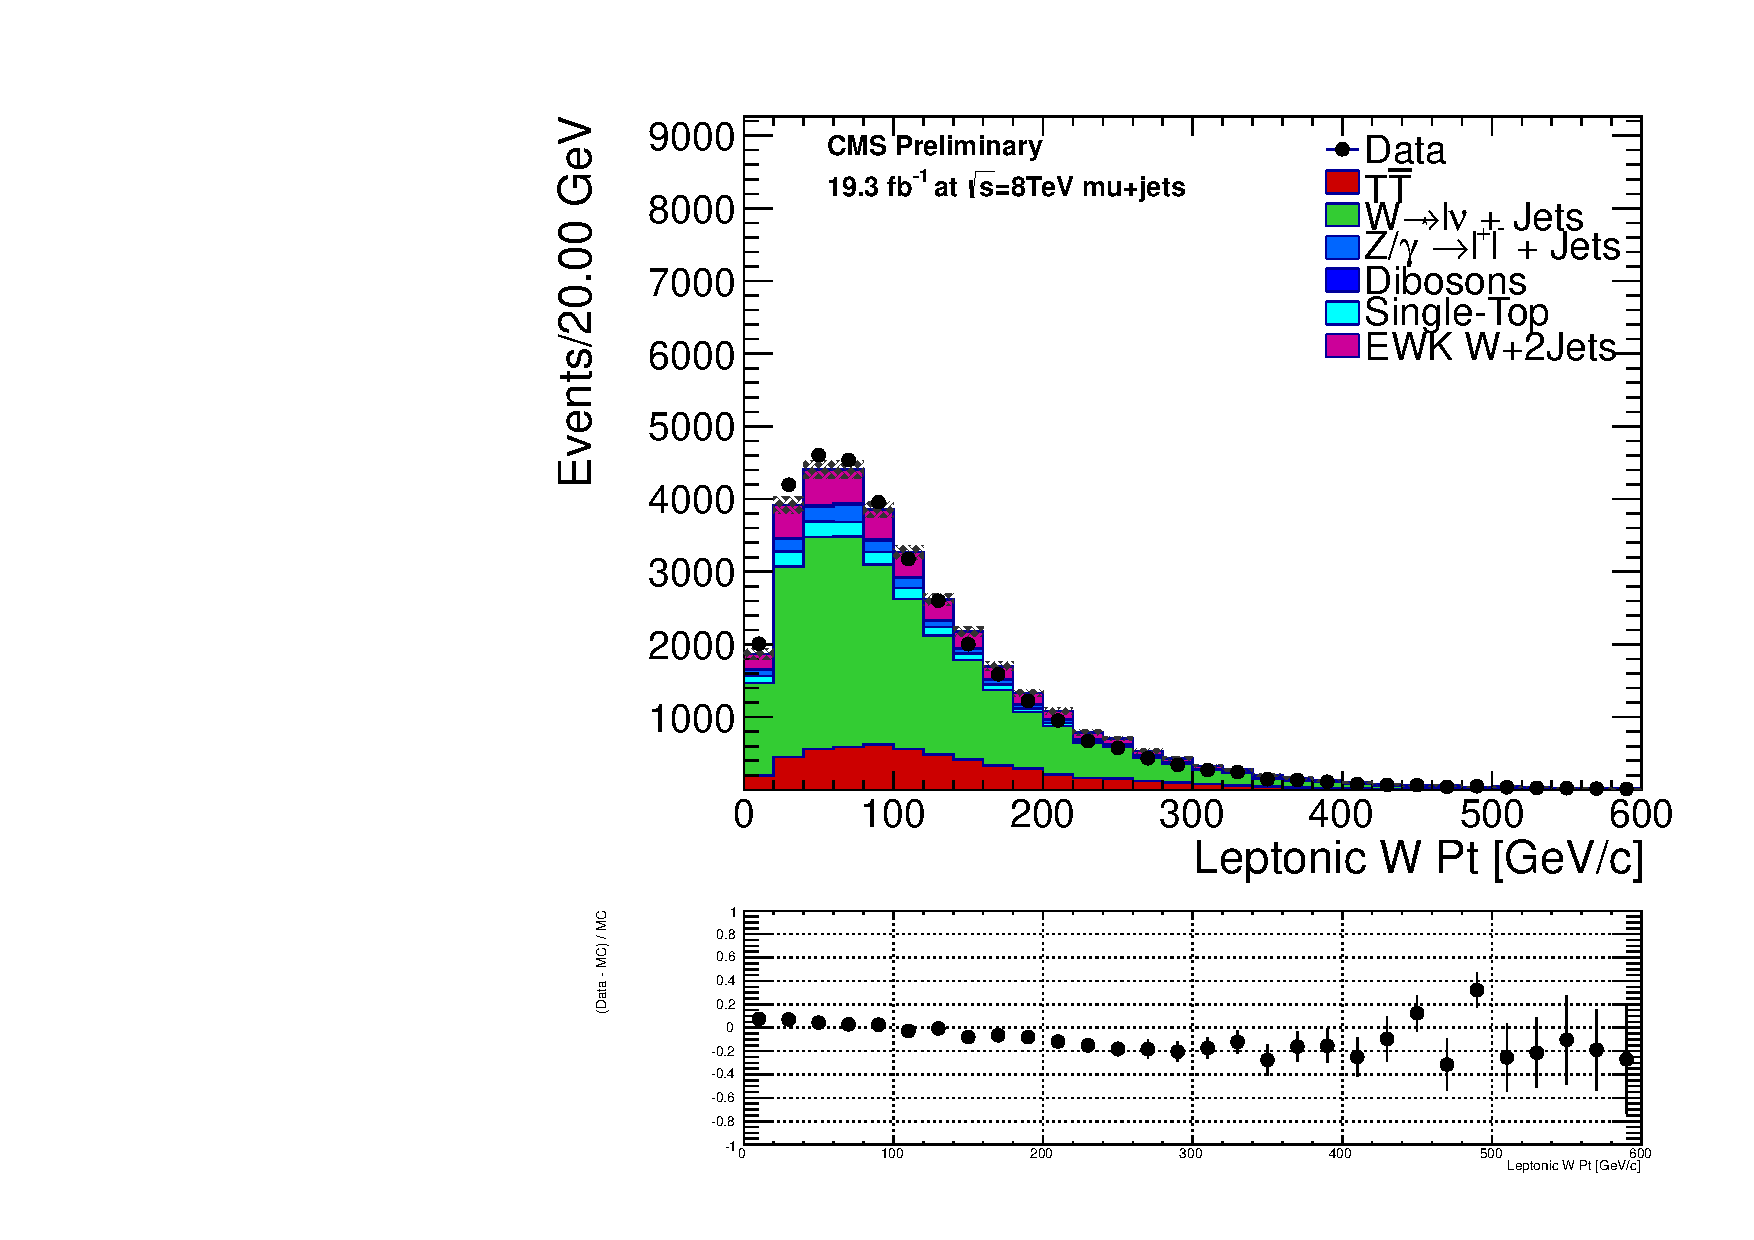
\includegraphics[width=.45\textwidth]{figs/n-1_plots_mu/mu_EWK_W_2jets_W_pt_mjj_600_tagjet1_60_tagjet2_50_Zeppenfield_1point2_EWKW2jets.pdf}
   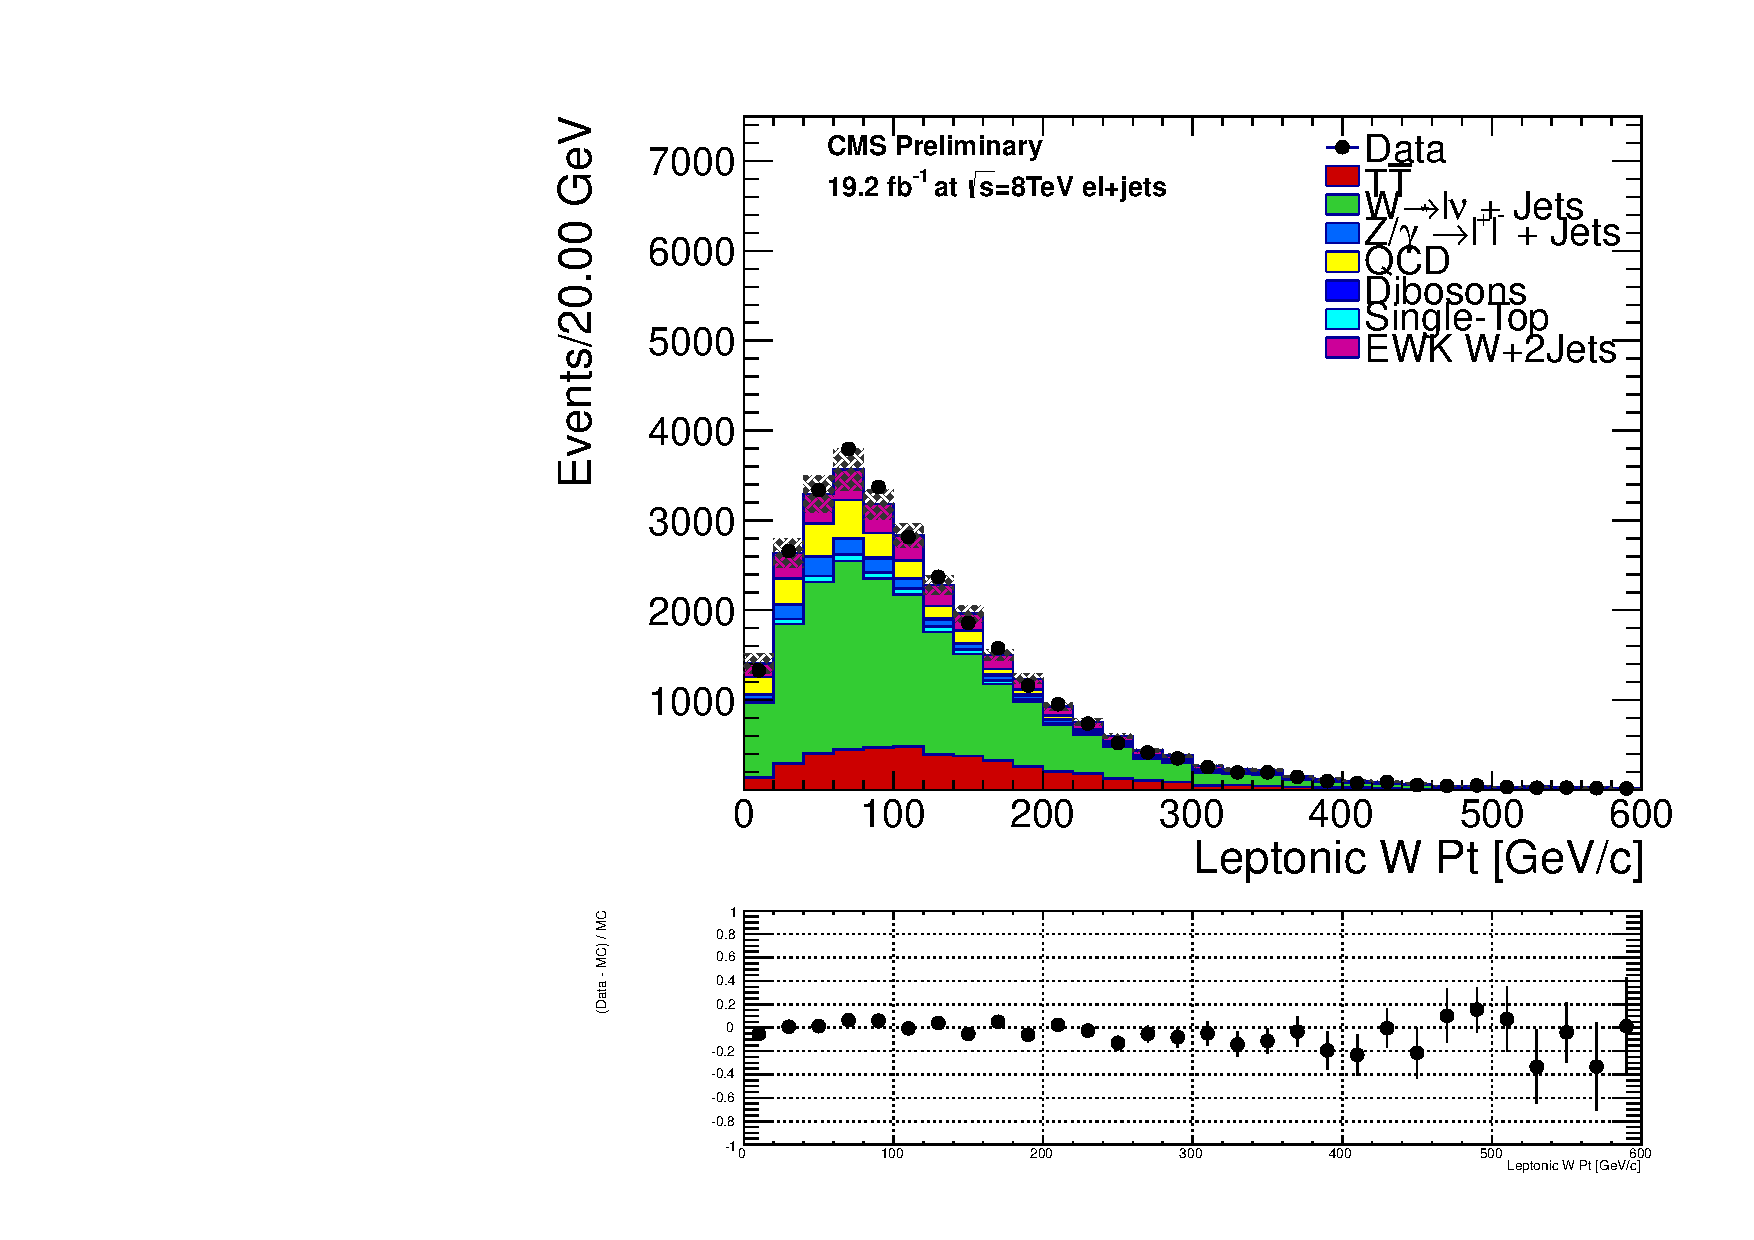
\includegraphics[width=.45\textwidth]{figs/n-1_plots_el/el_EWK_W_2jets_W_pt_mjj_600_tagjet1_60_tagjet2_50_Zeppenfield_1point2_met_30_WmT_30_EWKW2jets.pdf}
}
\caption{Distribution of leptonic W $p_{T}$ for muons (left) and electrons (right).}
\label{fig:lepw_pt}
\end{figure}

\begin{figure}[ht]
\centerline{
      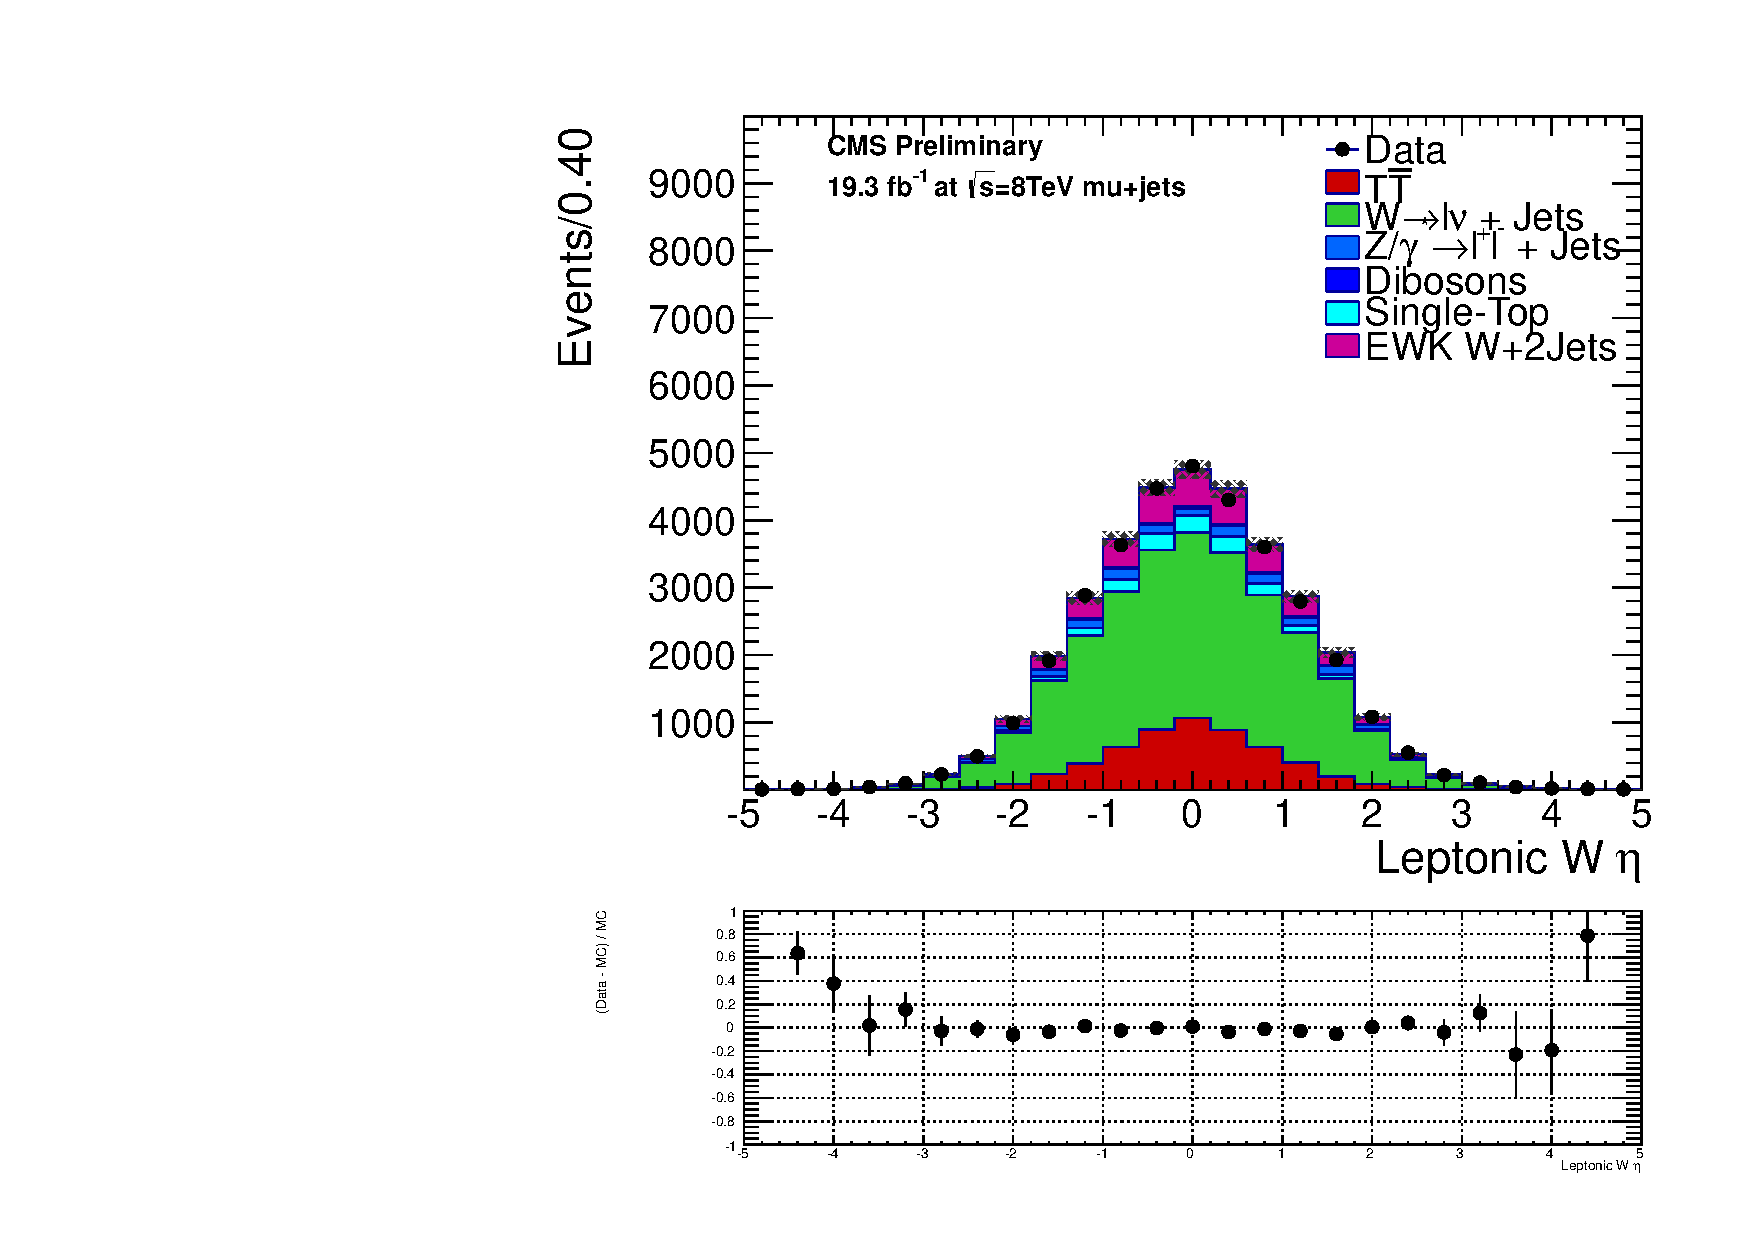
\includegraphics[width=.49\textwidth]{figs/n-1_plots_mu/mu_EWK_W_2jets_W_eta_mjj_600_tagjet1_60_tagjet2_50_Zeppenfield_1point2_EWKW2jets.pdf}
      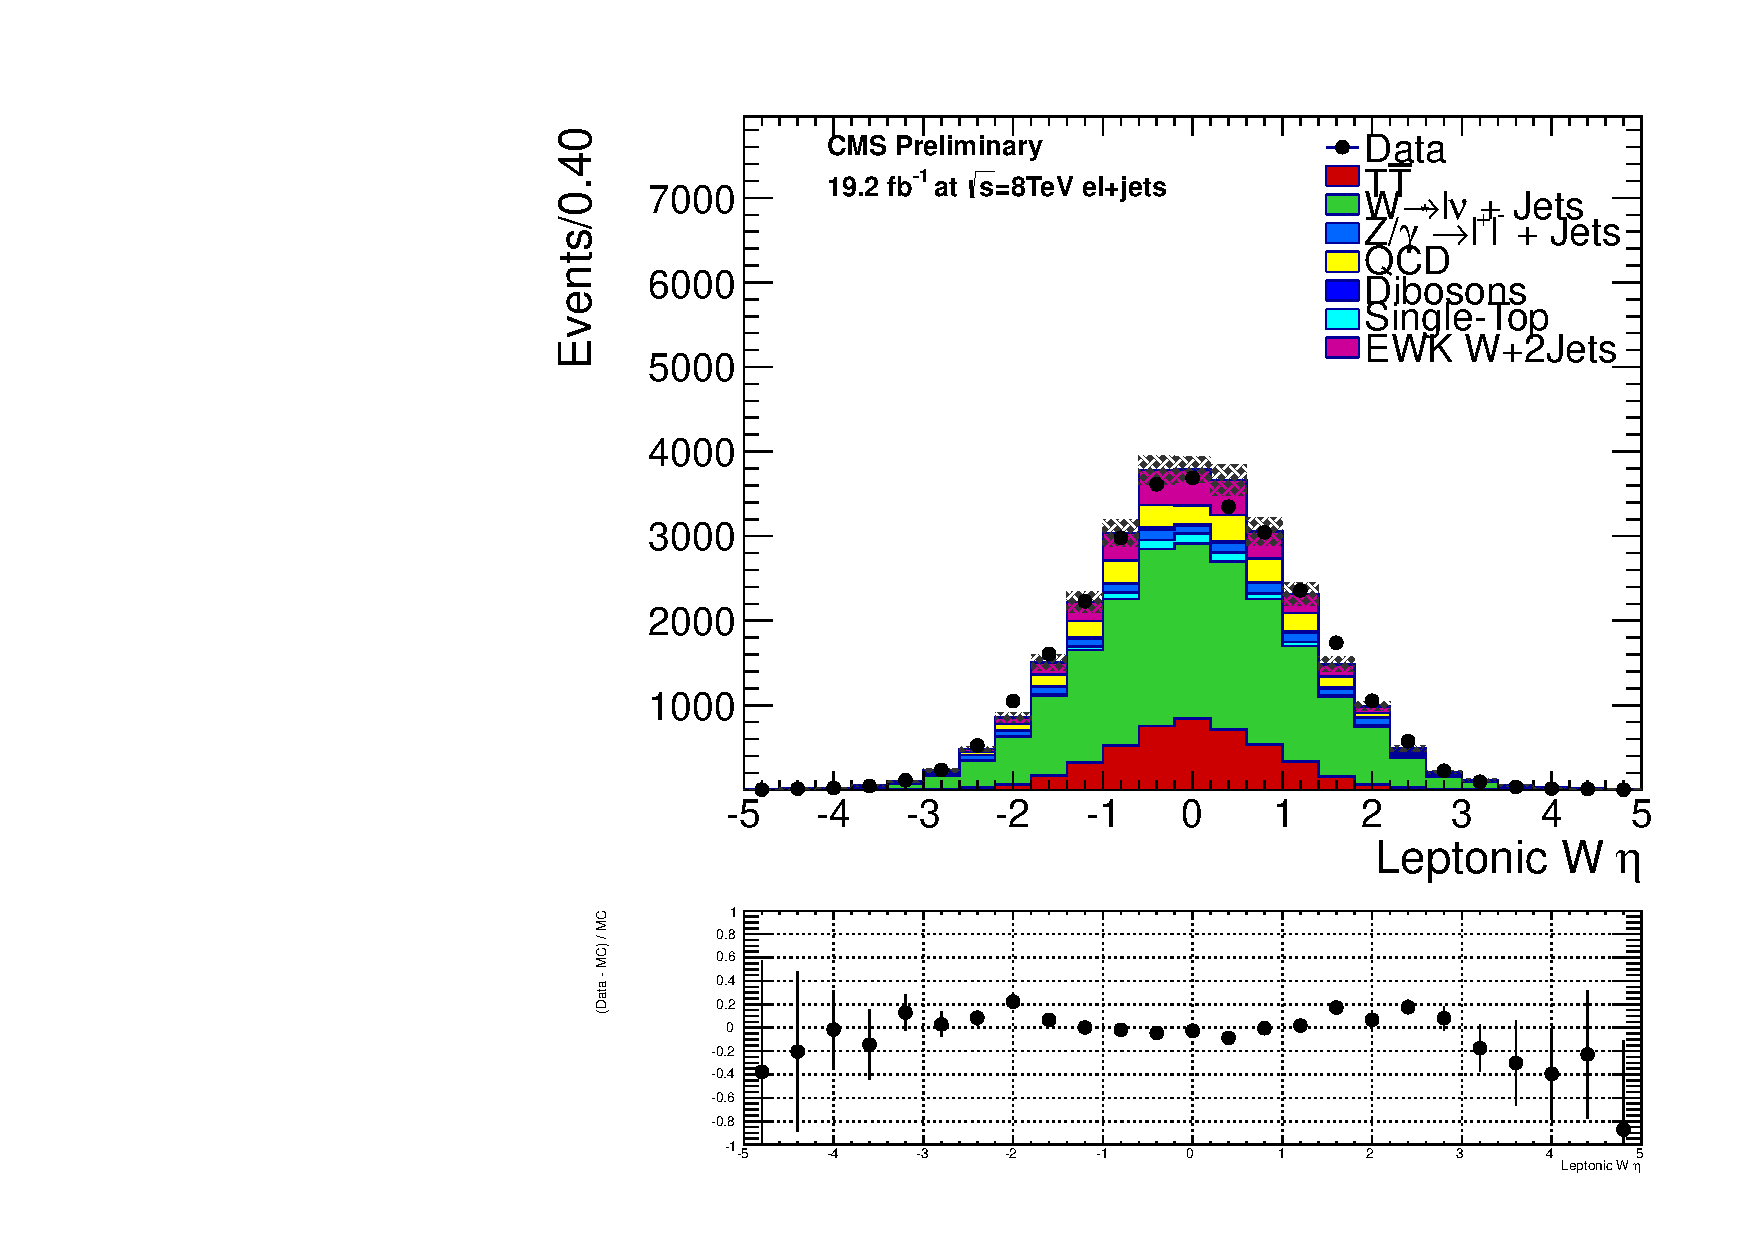
\includegraphics[width=.49\textwidth]{figs/n-1_plots_el/el_EWK_W_2jets_W_eta_mjj_600_tagjet1_60_tagjet2_50_Zeppenfield_1point2_met_30_WmT_30_EWKW2jets.pdf}
}
\caption{Distribution of leptonic W $\eta$ for muons (left) and electrons (right).}
\label{fig:lepw_eta}
\end{figure}

\begin{figure}[ht]
\centerline{
   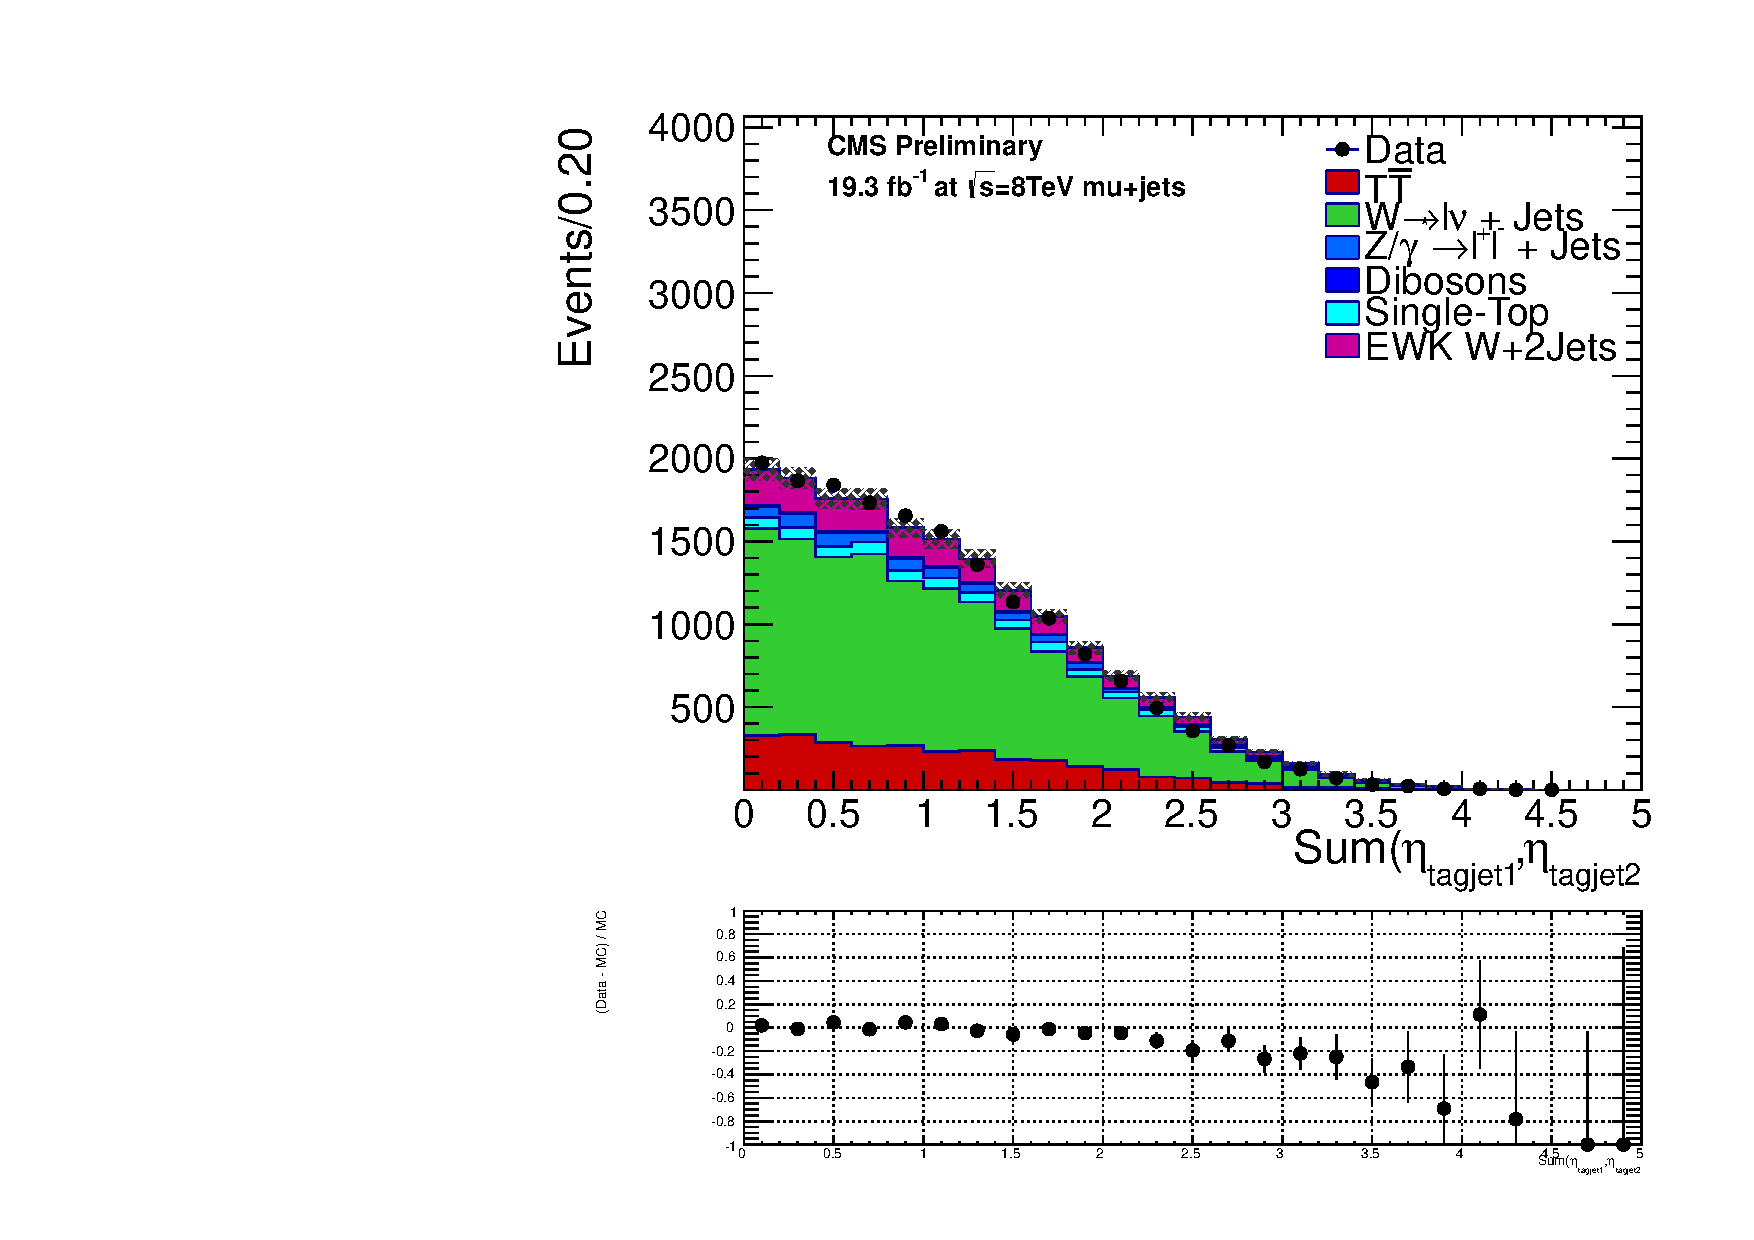
\includegraphics[width=.49\textwidth]{figs/n-1_plots_mu/mu_EWK_W_2jets_tagjet_sumeta_mjj_600_tagjet1_60_tagjet2_50_Zeppenfield_1point2_EWKW2jets.pdf}
   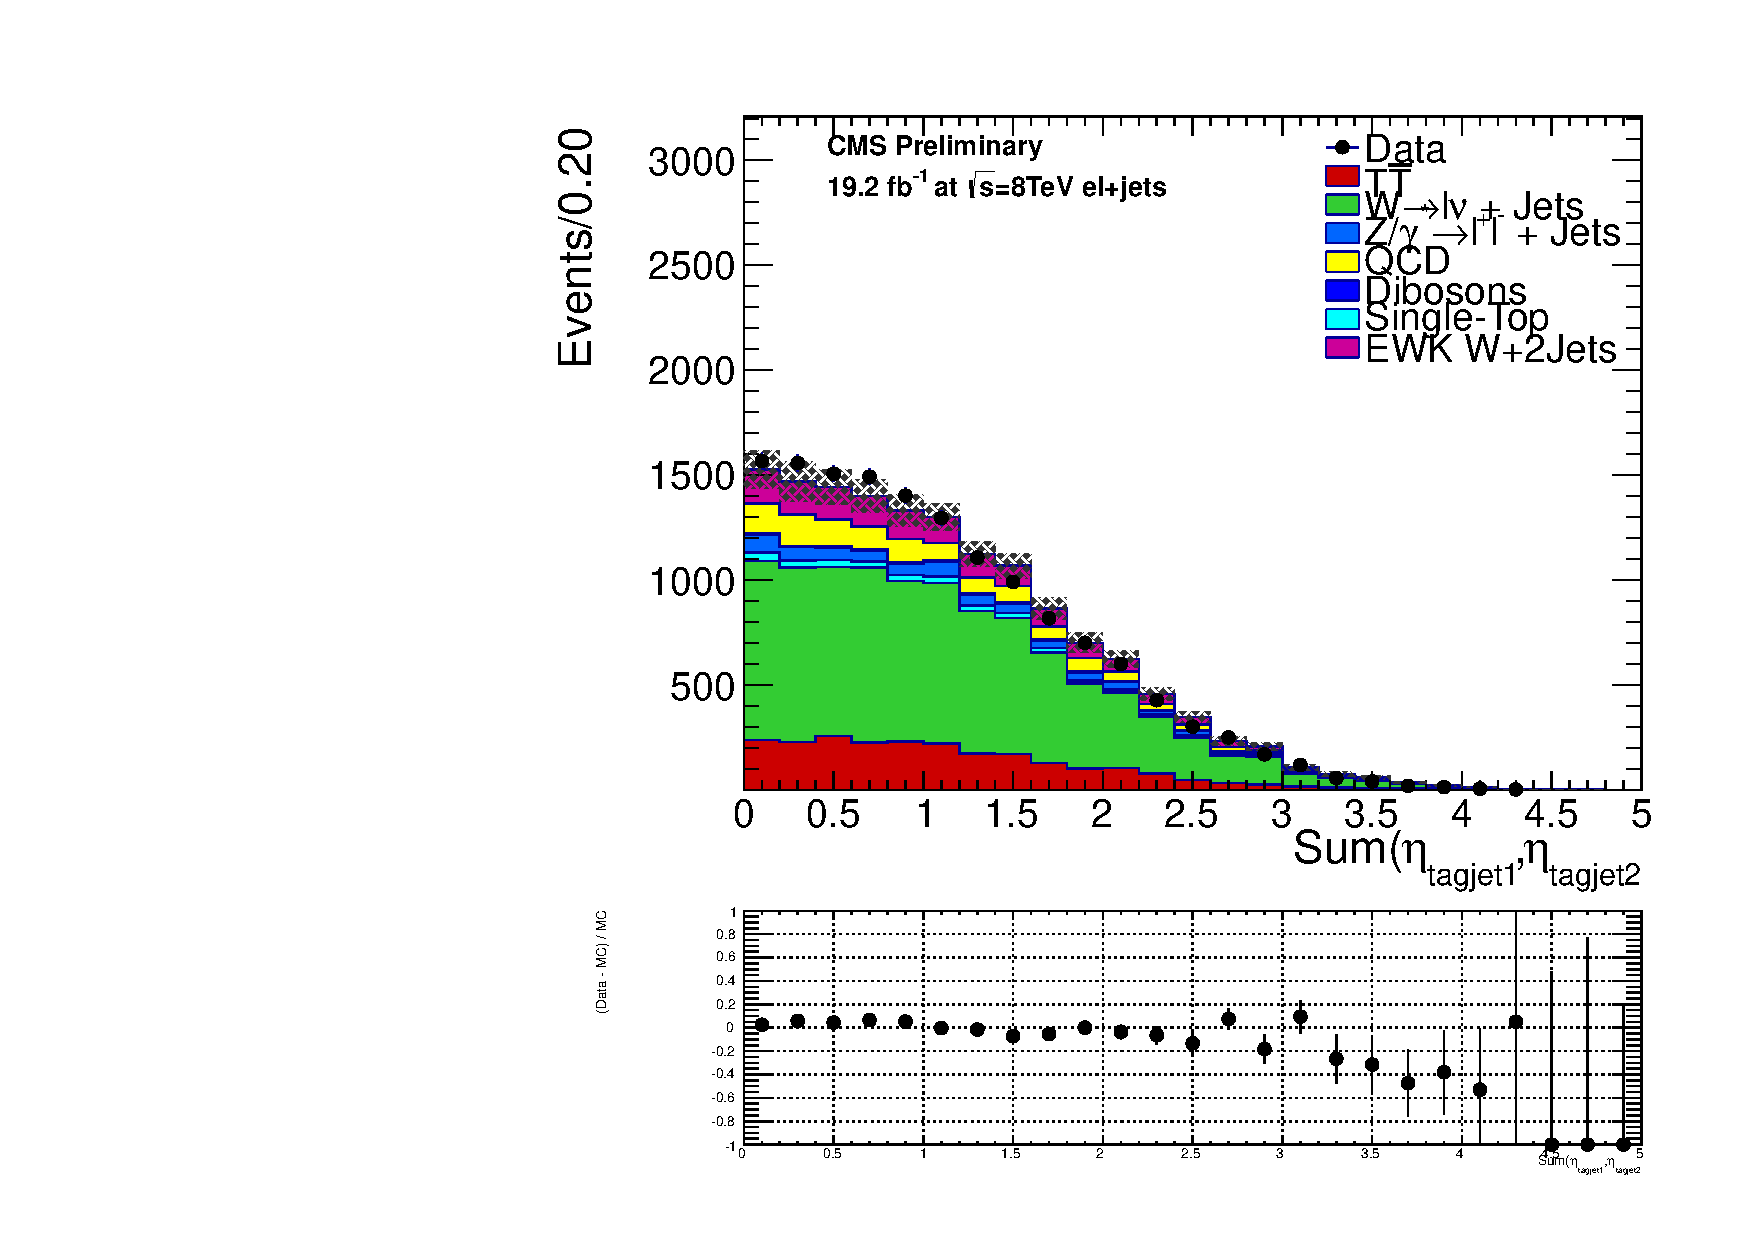
\includegraphics[width=.49\textwidth]{figs/n-1_plots_el/el_EWK_W_2jets_tagjet_sumeta_mjj_600_tagjet1_60_tagjet2_50_Zeppenfield_1point2_met_30_WmT_30_EWKW2jets.pdf}
}
\caption{Distribution of $\sum \eta(j1,j2)$ for muons (left) and electrons (right).}
\label{fig:sumeta}
\end{figure}

\begin{figure}[ht]
\centerline{
      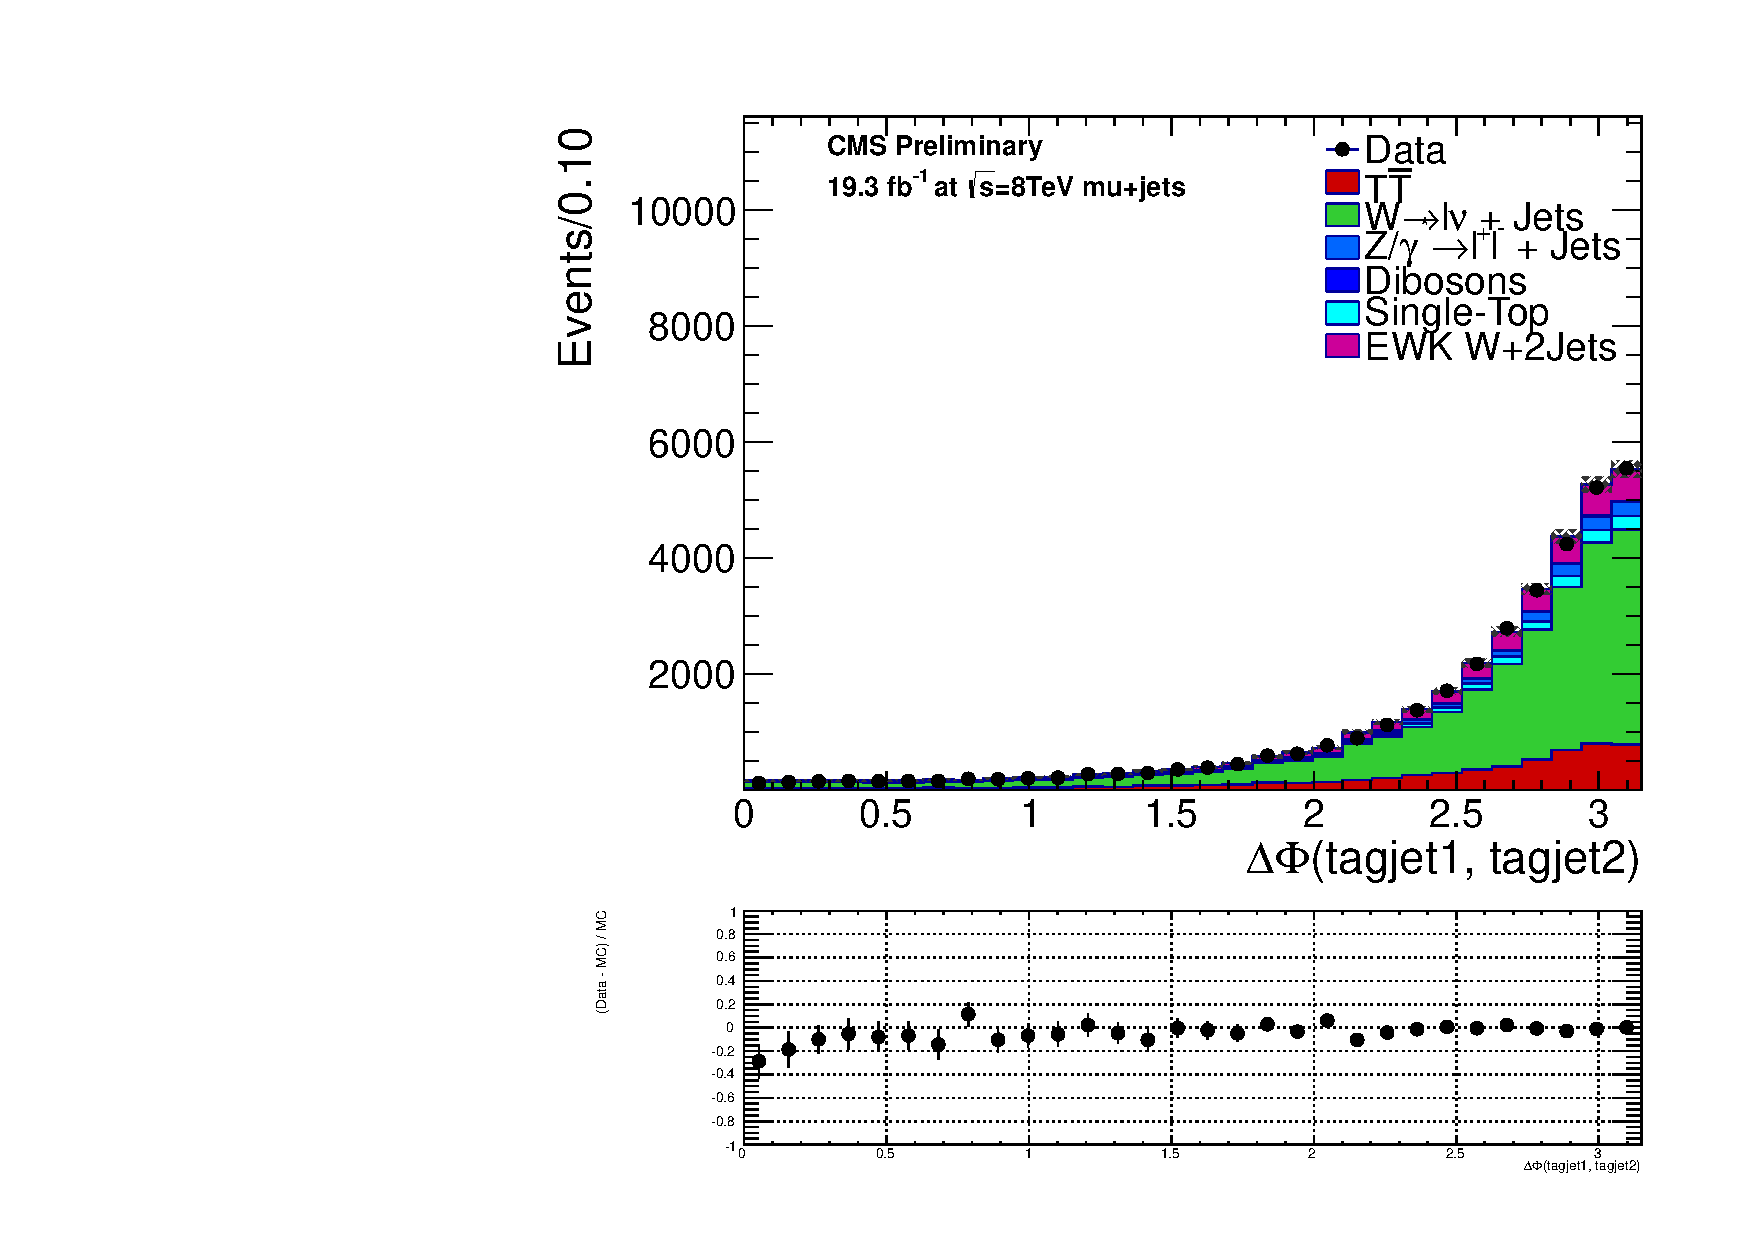
\includegraphics[width=.49\textwidth]{figs/n-1_plots_mu/mu_EWK_W_2jets_tagjet_deltaphi_mjj_600_tagjet1_60_tagjet2_50_Zeppenfield_1point2_EWKW2jets.pdf}
      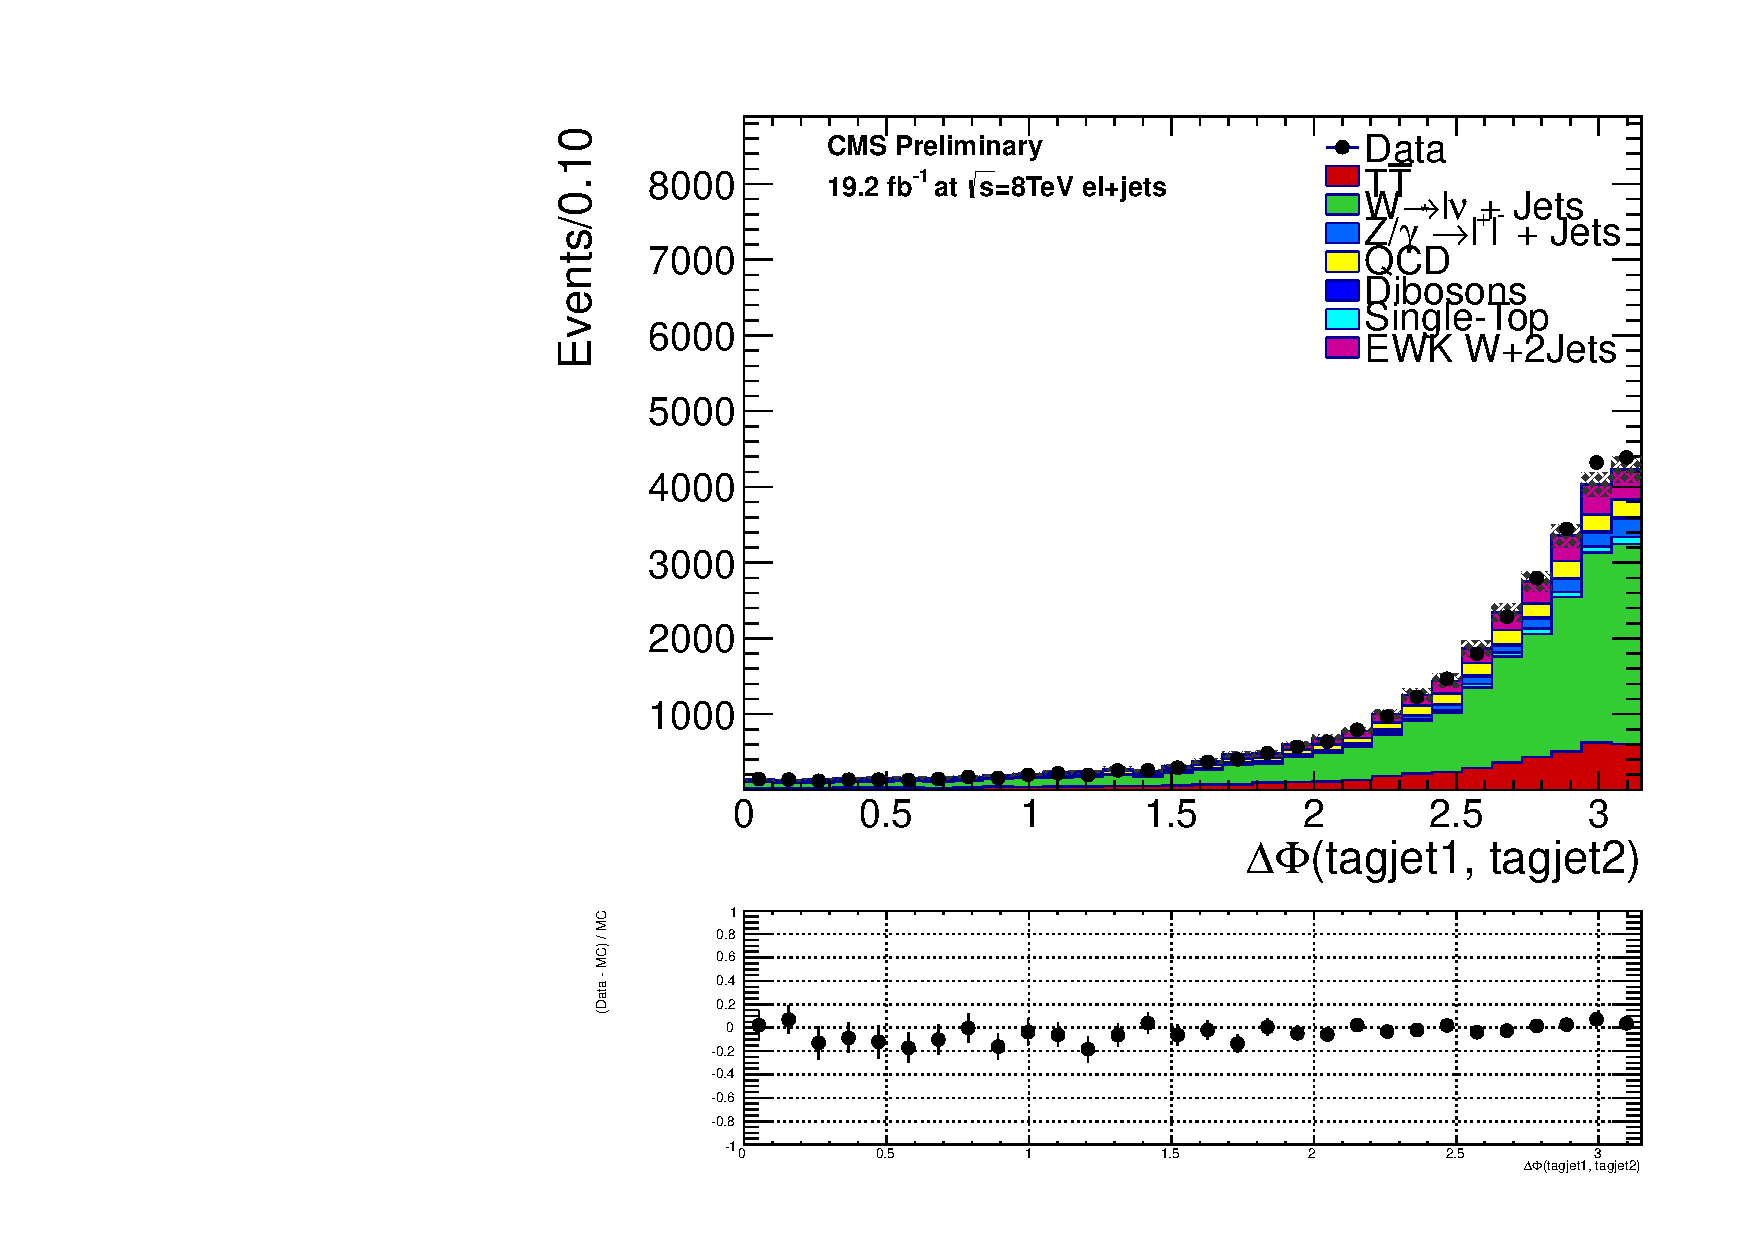
\includegraphics[width=.49\textwidth]{figs/n-1_plots_el/el_EWK_W_2jets_tagjet_deltaphi_mjj_600_tagjet1_60_tagjet2_50_Zeppenfield_1point2_met_30_WmT_30_EWKW2jets.pdf}
}
\caption{Distribution of $\Delta \phi(j1,j2)$ for muons (left) and electrons (right).}
\label{fig:deltaphij1j2}
\end{figure}

\begin{figure}[ht]
\centerline{
      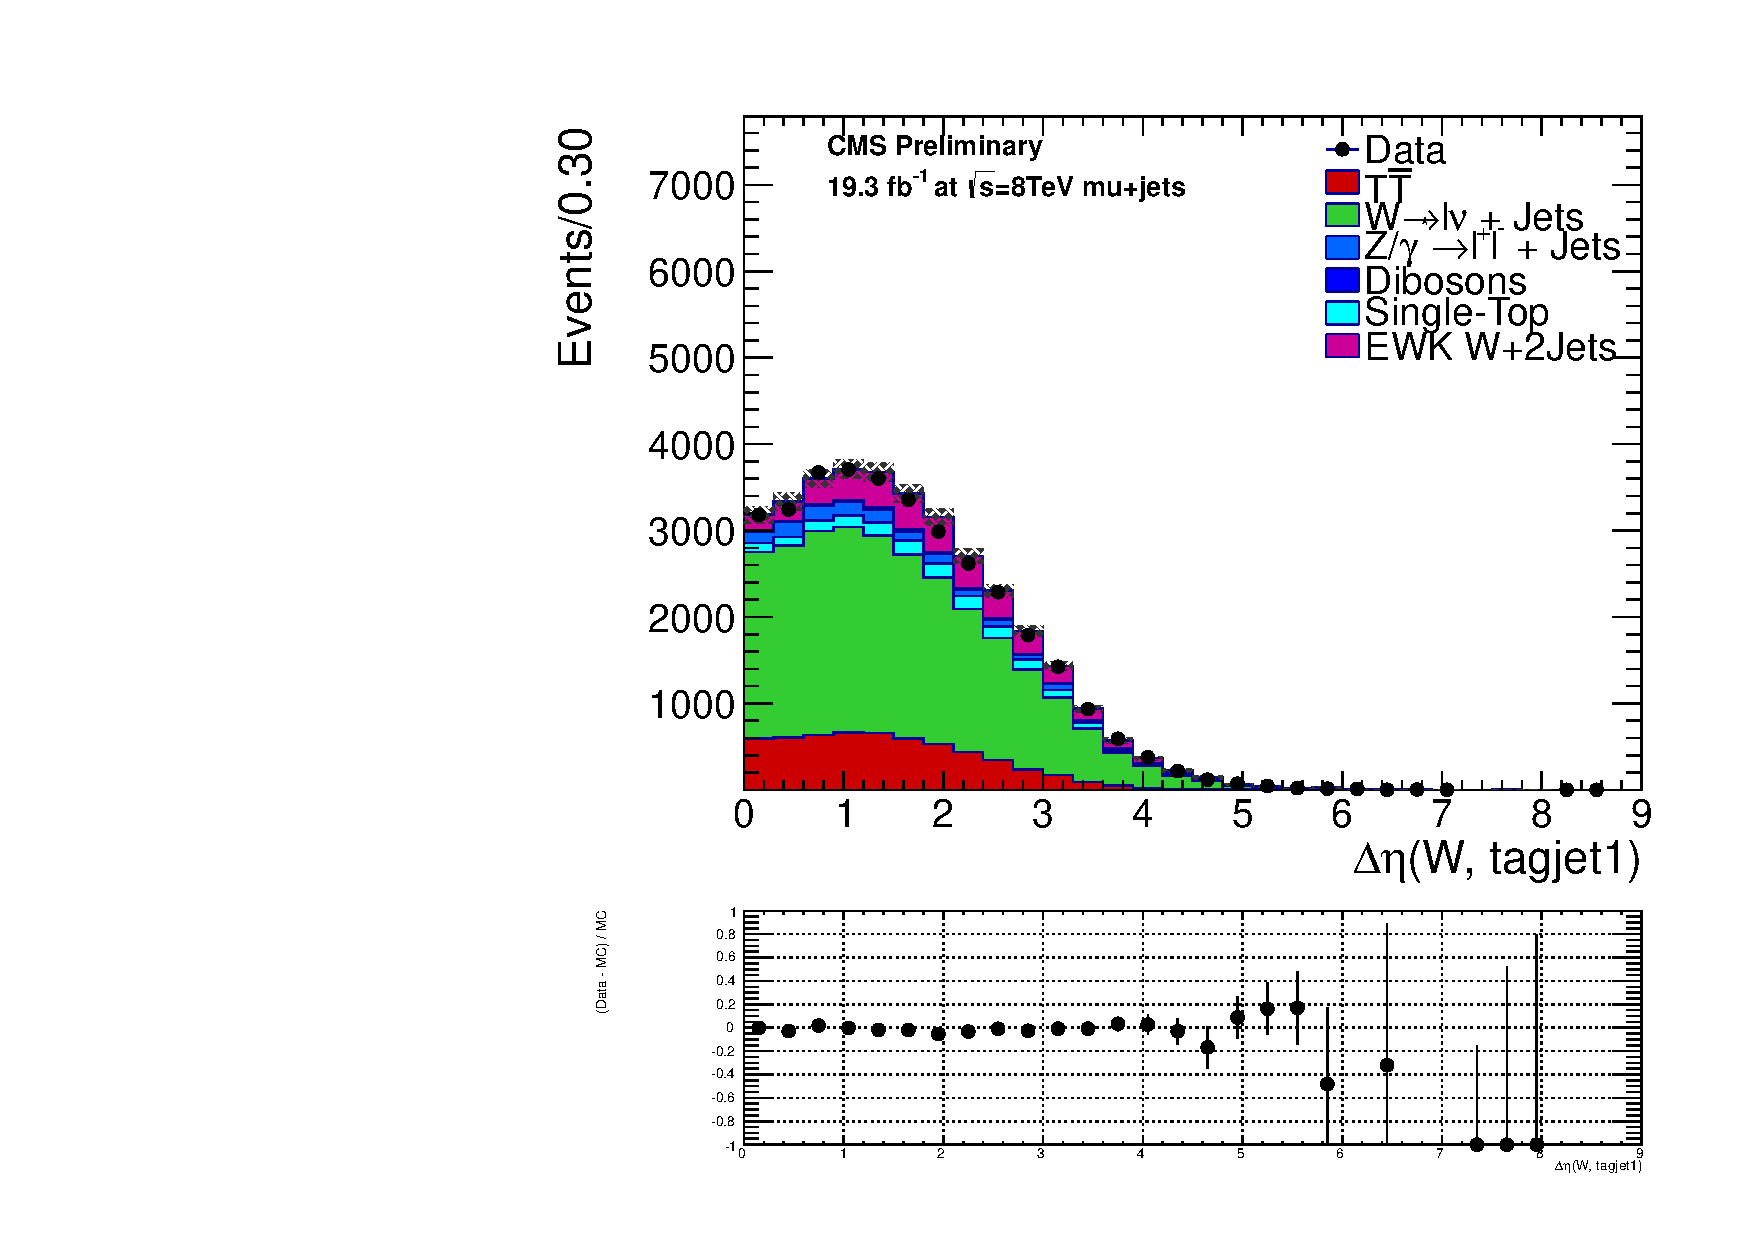
\includegraphics[width=.49\textwidth]{figs/n-1_plots_mu/mu_EWK_W_2jets_W_tagjet1_deltaeta_mjj_600_tagjet1_60_tagjet2_50_Zeppenfield_1point2_EWKW2jets.pdf}
      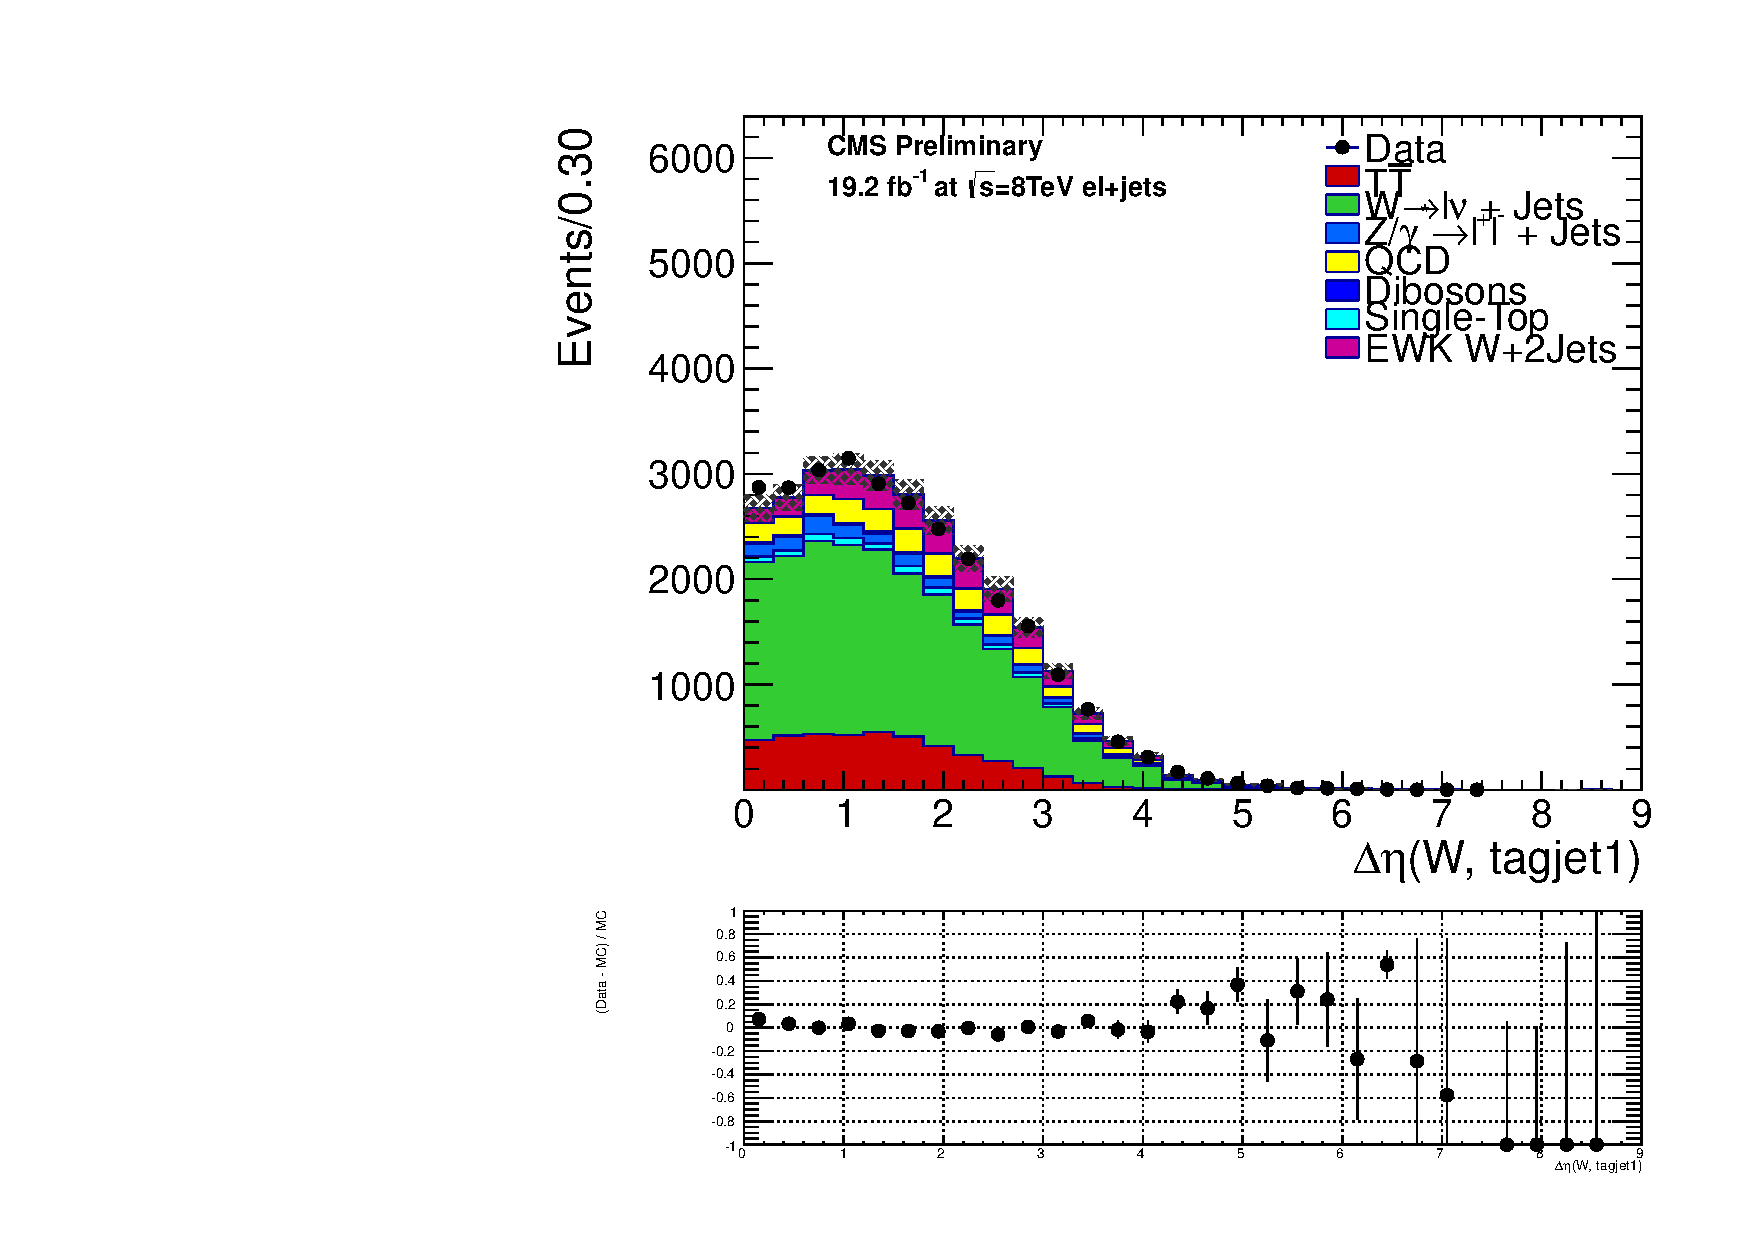
\includegraphics[width=.49\textwidth]{figs/n-1_plots_el/el_EWK_W_2jets_W_tagjet1_deltaeta_mjj_600_tagjet1_60_tagjet2_50_Zeppenfield_1point2_met_30_WmT_30_EWKW2jets.pdf}
}
\caption{Distribution of $\Delta \eta(W,j1)$ for muons (left) and electrons (right).}
\label{fig:deltaetawj1}
\end{figure}
%
%\clearpage
%\subsubsection{Selection of BDT Event Variables}
%The KS test quantification is done by using this test's implementation in  ROOT. It takes, as input, data and background distributions for a given variable, and returns a value between 0 and 1. A good variable for this analysis is considered to have a good KS test value. %of at least 0.10.
%
%After these criteria, we choose the best twenty six variables based on physics meaning, the BDT ranking variables output, and the shape of the distributions.  The most powerful variables for the \gh model and the \ft SM, taken from the BDT ranking variables output given by TMVA, are: $S_T^{\rm jet}$, number of jets, leading jet $\eta$, \MET, second leading jet $\eta$ and $\Delta R (j1,j2)$. Some variables are more important for the lower mass \gh than the high mass \gh, or for the \ft SM, therefore we keep a large number of variables trying to keep as much information about the event as possible. 
%%A list of all variables considered for this analysis is shown in Table \ref{tab:KSvariables}. Although some non-considered variables have a good KS value, they have a bad performance for the training method. 
%Distributions for the variables used in the BDT training are shown in Figures \ref{fig:Stjet}-\ref{fig:deltaPhilepnu}. In order to maximize the information and keep the training method optimized, the variables with highest correlations are not selected. Figure~\ref{fig:correlation_matrix} shows an example of a correlation matrix for the variables used in the case of the \muons channel for the \gh mass of 0.6 TeV (for other mass points and for the \electrons channel, this matrix is very similar).

%We also compare the shape of the distribution of these variables between a sample of \ttbar generated in Madgraph and other generated in Powheg. More details about this comparison and these distributions are shown in the Appendix~\ref{app:ttbarcompare}. We found good agreement between these two ttbar samples.

\begin{figure}[ht]
\centerline{
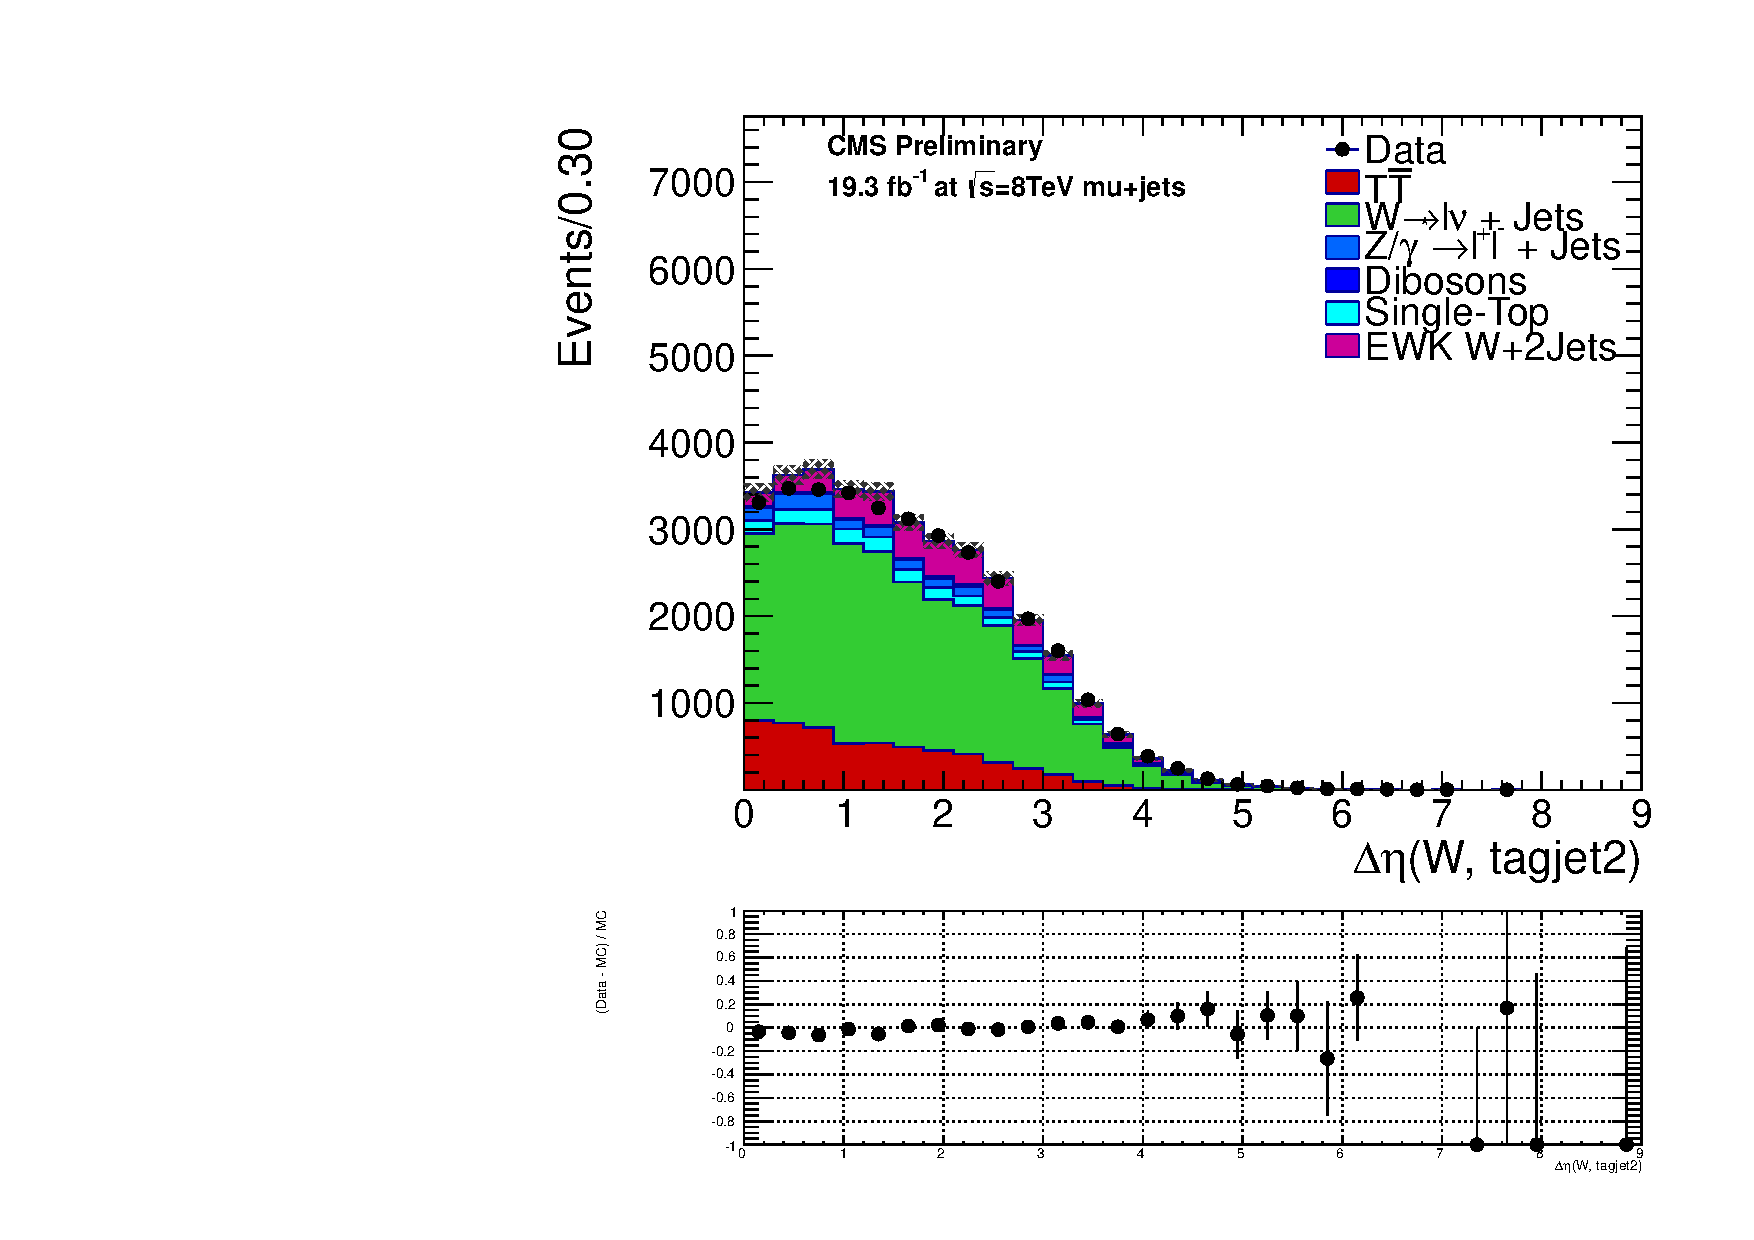
\includegraphics[width=.49\textwidth]{figs/n-1_plots_mu/mu_EWK_W_2jets_W_tagjet2_deltaeta_mjj_600_tagjet1_60_tagjet2_50_Zeppenfield_1point2_EWKW2jets.pdf}
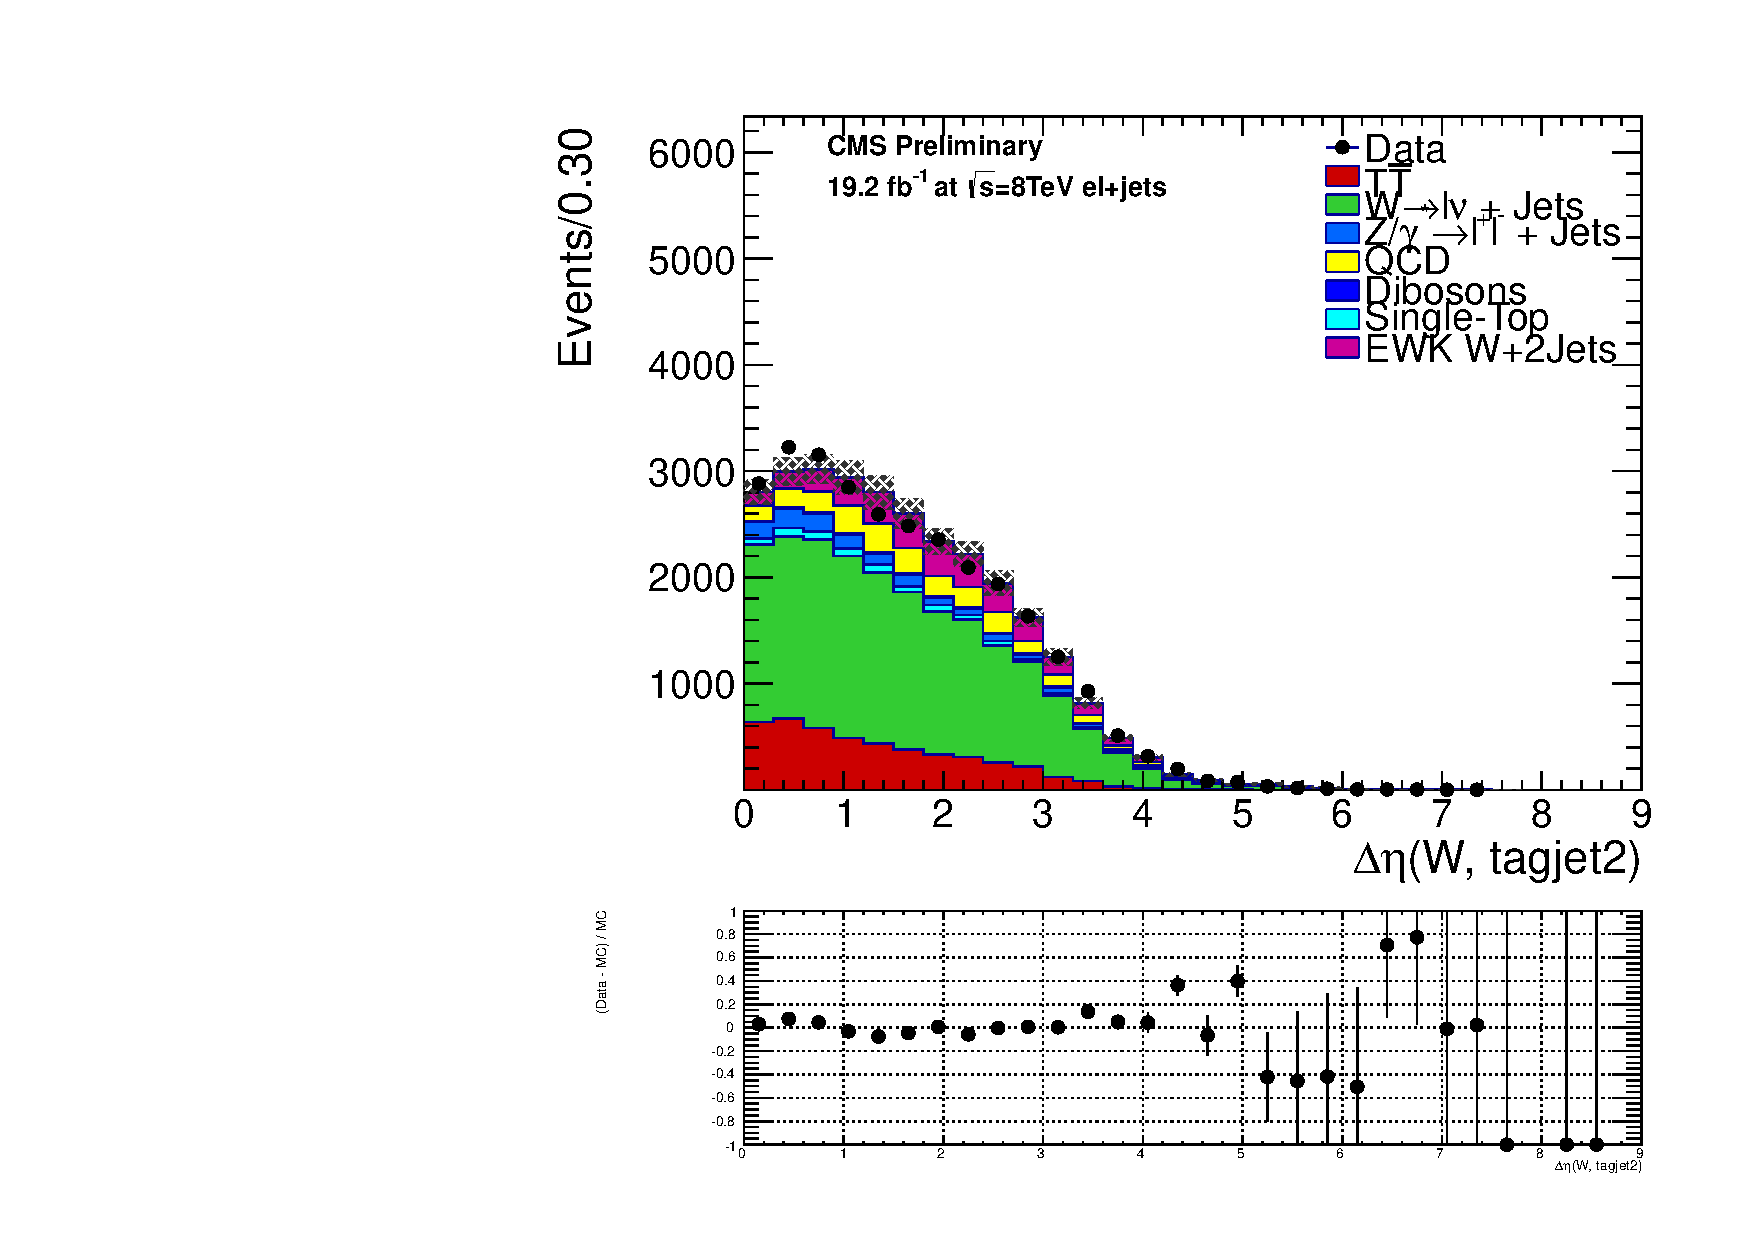
\includegraphics[width=.49\textwidth]{figs/n-1_plots_el/el_EWK_W_2jets_W_tagjet2_deltaeta_mjj_600_tagjet1_60_tagjet2_50_Zeppenfield_1point2_met_30_WmT_30_EWKW2jets.pdf}
}
\caption{Distribution of $\Delta \eta(W,j2)$ for muons (left) and electrons (right).}
\label{fig:deltaetawj2}
\end{figure}

\begin{figure}[ht]
\centerline{
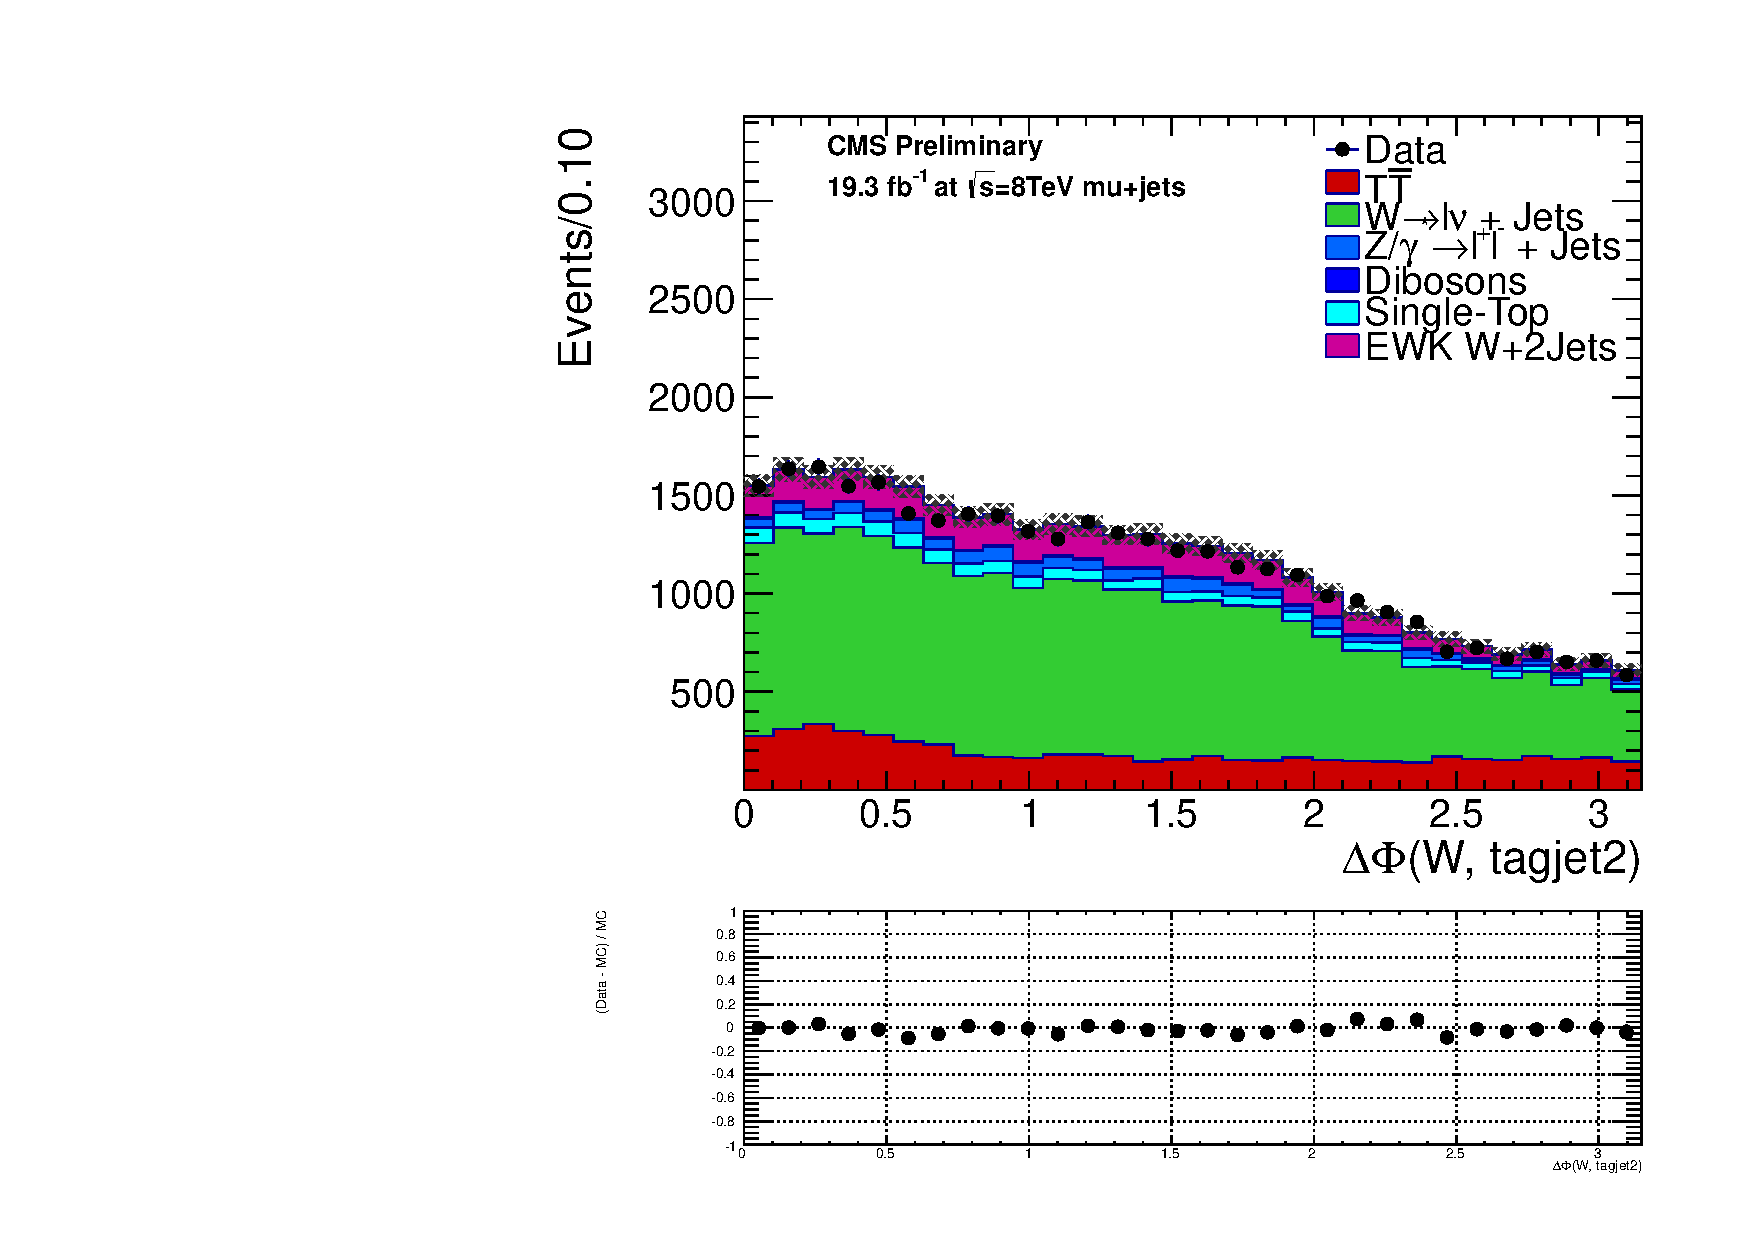
\includegraphics[width=.49\textwidth]{figs/n-1_plots_mu/mu_EWK_W_2jets_W_tagjet2_deltaphi_mjj_600_tagjet1_60_tagjet2_50_Zeppenfield_1point2_EWKW2jets.pdf}
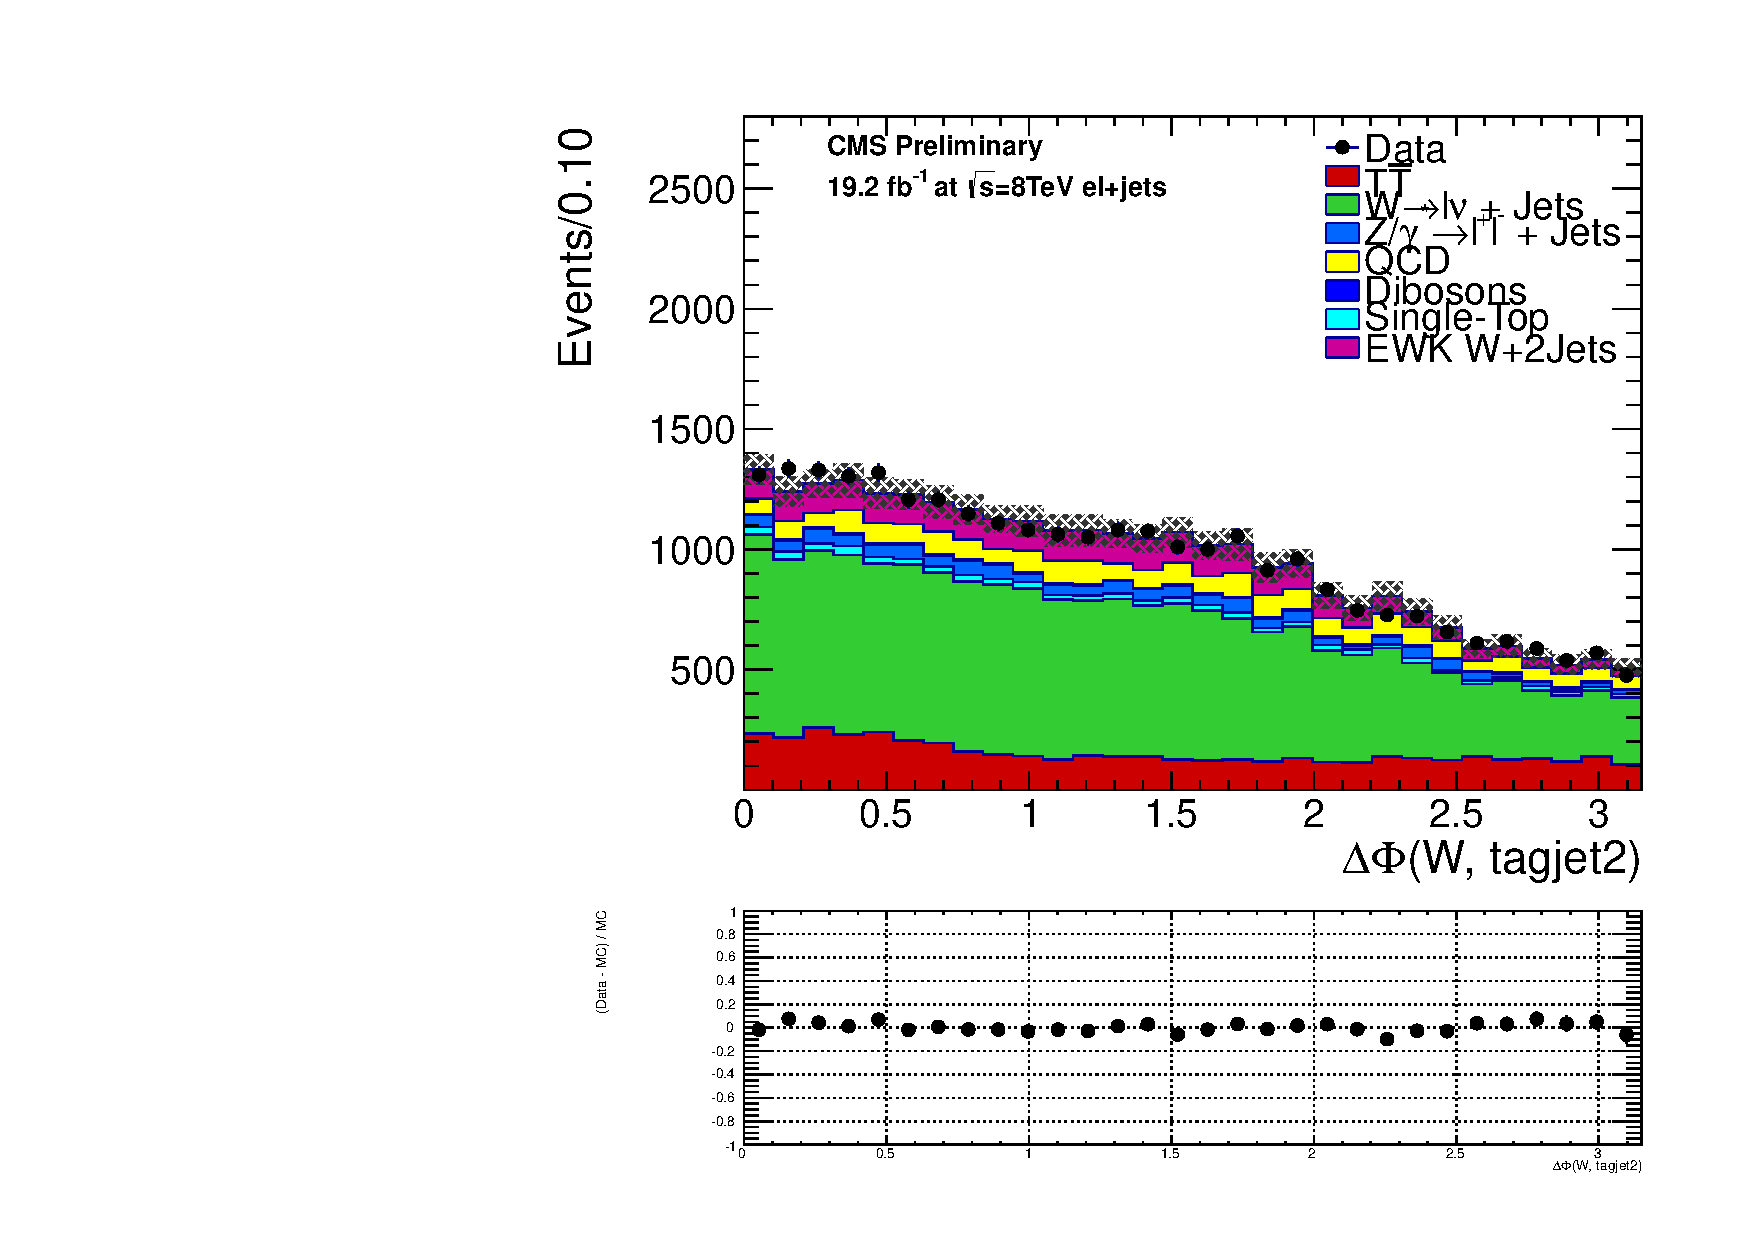
\includegraphics[width=.49\textwidth]{figs/n-1_plots_el/el_EWK_W_2jets_W_tagjet2_deltaphi_mjj_600_tagjet1_60_tagjet2_50_Zeppenfield_1point2_met_30_WmT_30_EWKW2jets.pdf}
}
\caption{Distribution of $\Delta \phi(W,j2)$ for muons (left) and electrons (right).}
\label{fig:deltaphiwj2}
\end{figure}

%\begin{figure}[ht]
%\centerline{
%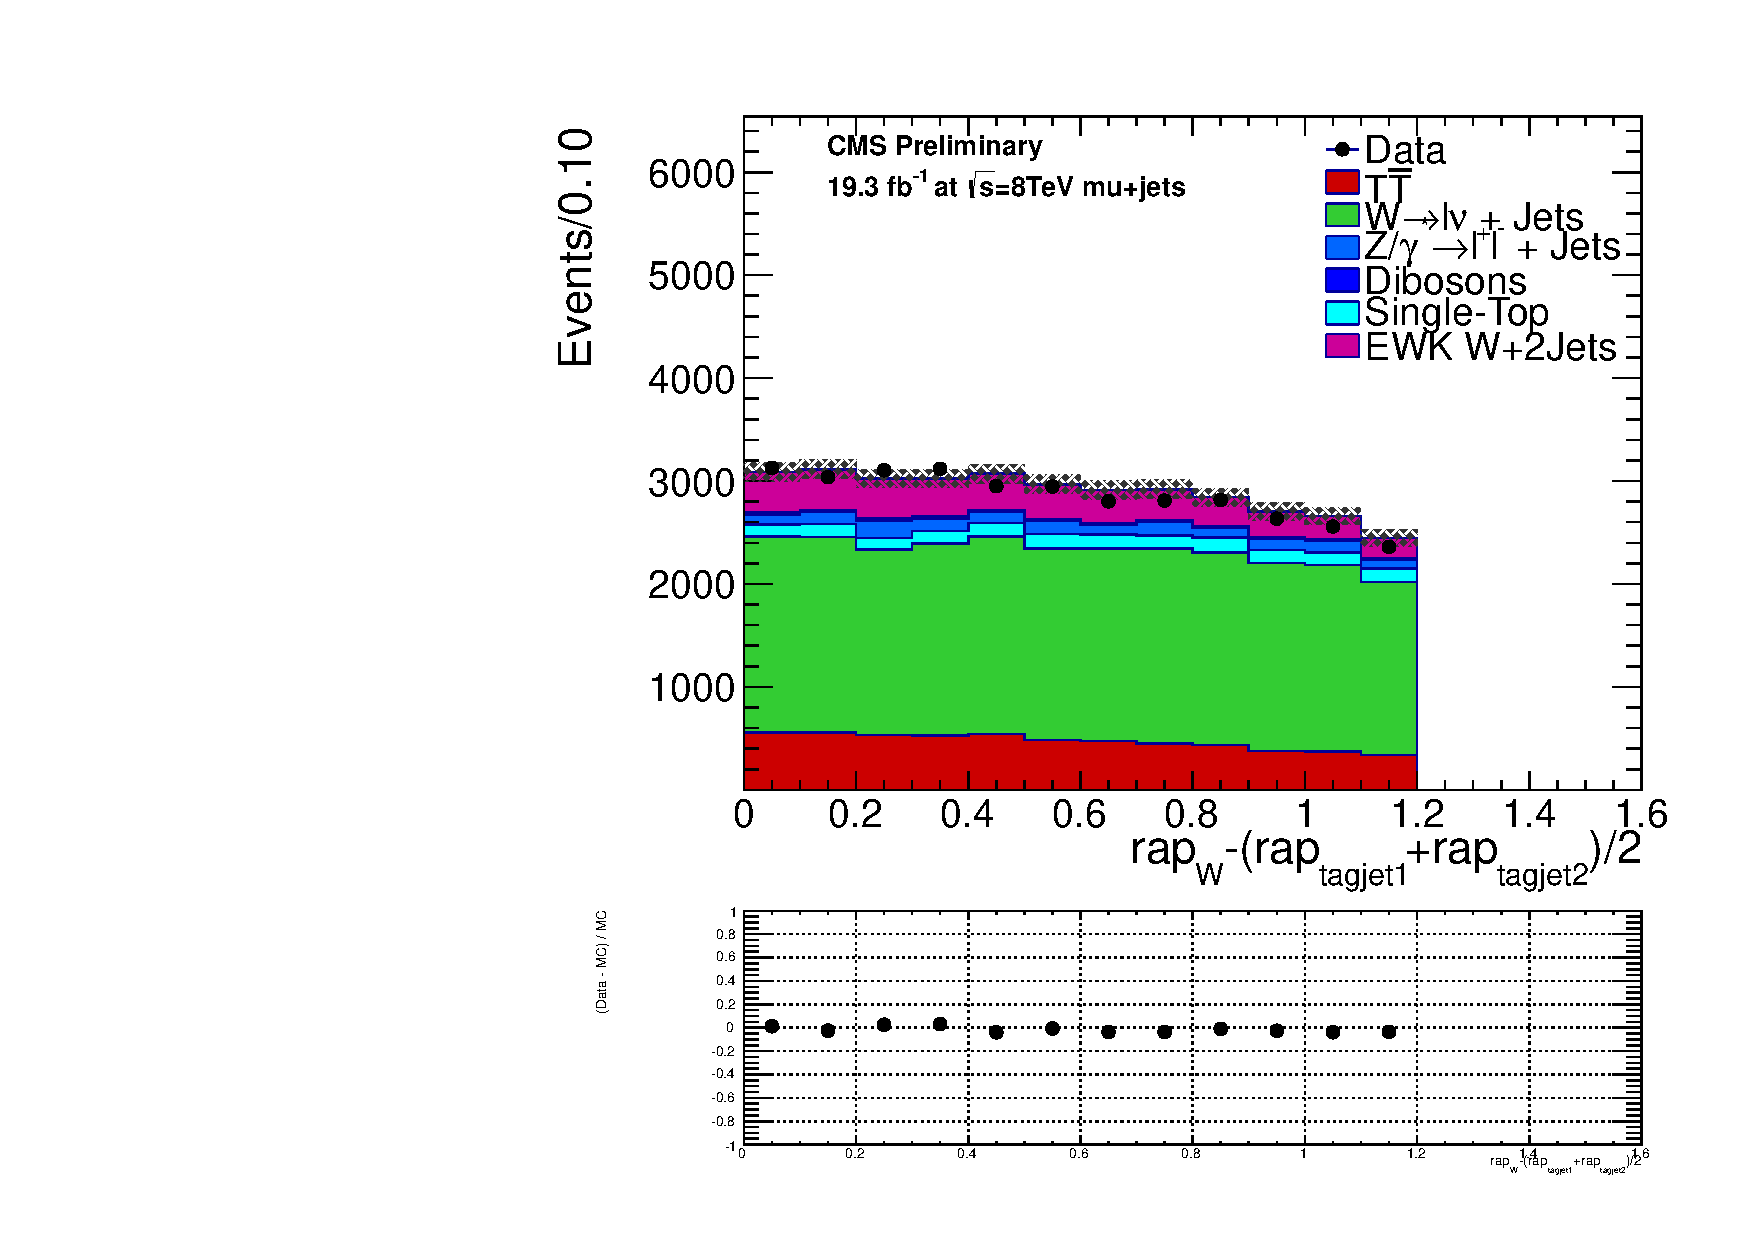
\includegraphics[width=.49\textwidth]{figs/n-1_plots_mu/mu_EWK_W_2jets_W_tagjet_Zeppenfield_mjj_600_tagjet1_60_tagjet2_50_Zeppenfield_1point2_EWKW2jets.pdf}
%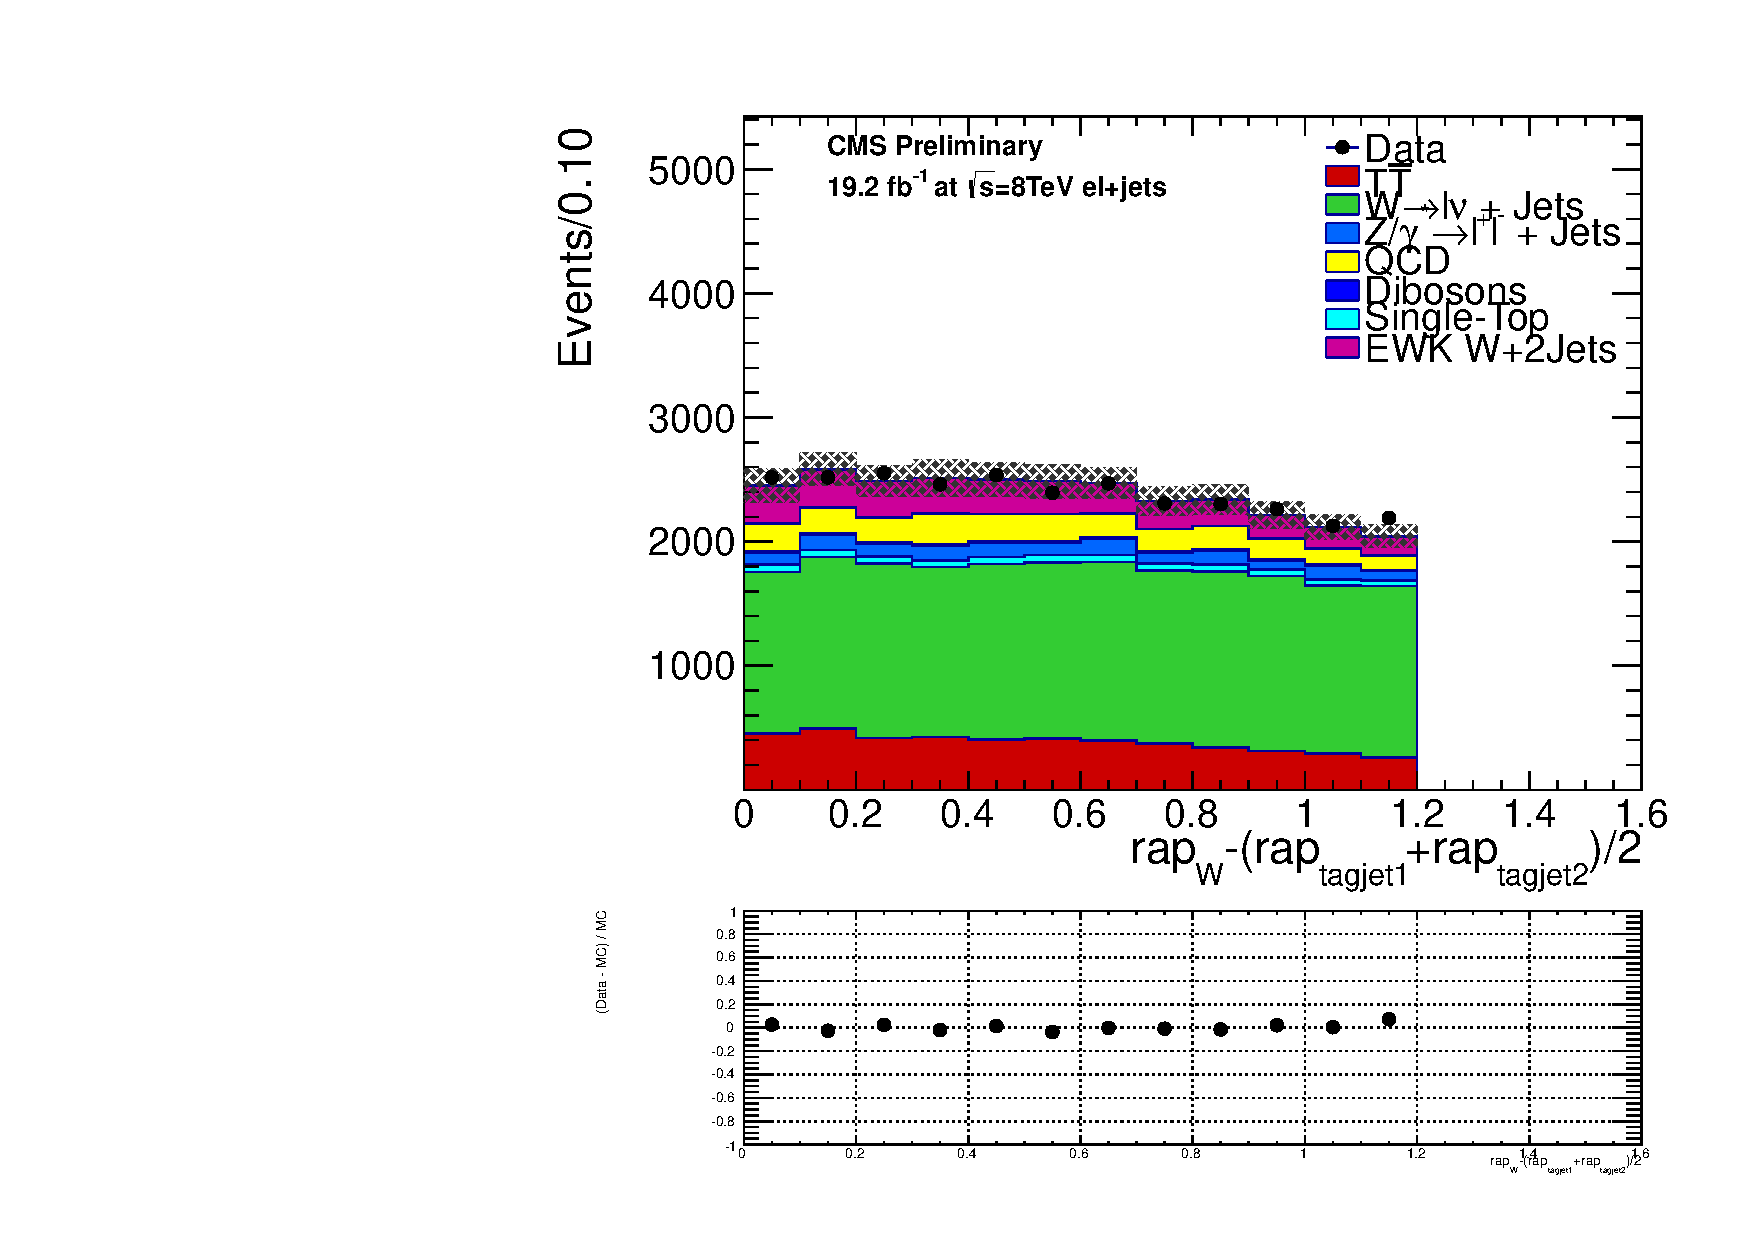
\includegraphics[width=.49\textwidth]{figs/n-1_plots_el/el_EWK_W_2jets_W_tagjet_Zeppenfield_mjj_600_tagjet1_60_tagjet2_50_Zeppenfield_1point2_met_30_WmT_30_EWKW2jets.pdf}
%}
%\caption{Distribution of the Zeppenfeld variable for muons (left) and electrons (right).}
%\label{fig:zeppenfield}
%\end{figure}

\clearpage

\subsection{BDT Output Distribution}
We train the BDT using the variables described in Table \ref{tab:objkin} to Table \ref{tab:recoangu}. Because our dominant background is W+jets, we only use this sample for the BDT training in the muons and the electrons channels. 
%The BDT training setup is tunned with the value given by the testing efficiency compared to training efficiency at 0.01 of background. This value is reported by TMVA. In both channels the signal efficiency is greater than 0.5 for the test and training samples. 

We use the Adaptive Boost Algorithm (AdaBoost) \cite{Freund:1997:DGO:261540.261549} with the AdaBoostBeta = 1 and 400 trees for training. We apply the CrossEntropy as separation criterion for node splitting, then we require at least 400 events in a leaf node and nCuts=20 for the number of steps for BDT training. 
%These BDT parameters are optimized using the \gh mass point of 600. Overtraining problems have been reduced by using these BDT parameters. The detailed cross check of BDT can be found in the Appendix~\ref{app:bdt_crosscheck}.%This invokes an algorithm, in the TMVA package, that tests all possible cuts on the training sample and finds the best one.
%In order to maximize the information and keep the training method optimized, the variables with highest correlations are not selected. 
Figure~\ref{fig:correlation_matrix} shows an example of a correlation matrix for the variables used in the training.
%Figure \ref{fig:correlation_matrix} shows the Correlation Matrix according to TMVA for the eight variables used in this analysis. 
Additionally, we compare the data and background distributions for BDT output. Figures \ref{fig:BDToutputdistribution} shows the BDT output distributions for muons and electrons events. EWK W+2jets signal is clear to see in the high side of BDT output distribution. %These BDT output distributions are used to set the \gh mass limit.

%The BDT output distribution will be used in two ways:
%\begin{itemize}
%\item By applying the reverse BDT cut($<$ 0.1), we calculate Wjets normalization scale factor by fitting to data in this Wjets dominant region. In this fit, we fix other background process(Top, Z+Jets,Diboson) contribution. The fit result can be found in Table~\ref{tab:bdtfitcontrol}.Then we apply this Wjets normalization scale factor in the later tag jet pair invariant mass fit and BDT output distribution signal region($>$ 0.1) fit.
%\item We directly use the BDT signal region($>$ 0.1) output shape to calculate the electroweak W+2jets signal cross section. In this fit, we fix the Wjets normalization scale factor from the previous step and other minor background contribution(ZJets and Diboson). Then we float the Top(TTbar+SingleTop) and EWKW2jets signal contribution. This is the cross check result with tagjet pair $m_{jj}$ distribution fit. The signal strength fit result can be found in Table~\ref{tab:bdtfitresult}. We found consisted fit result between these two methods.
%
\end{itemize}

\begin{figure}[ht]
\centerline{
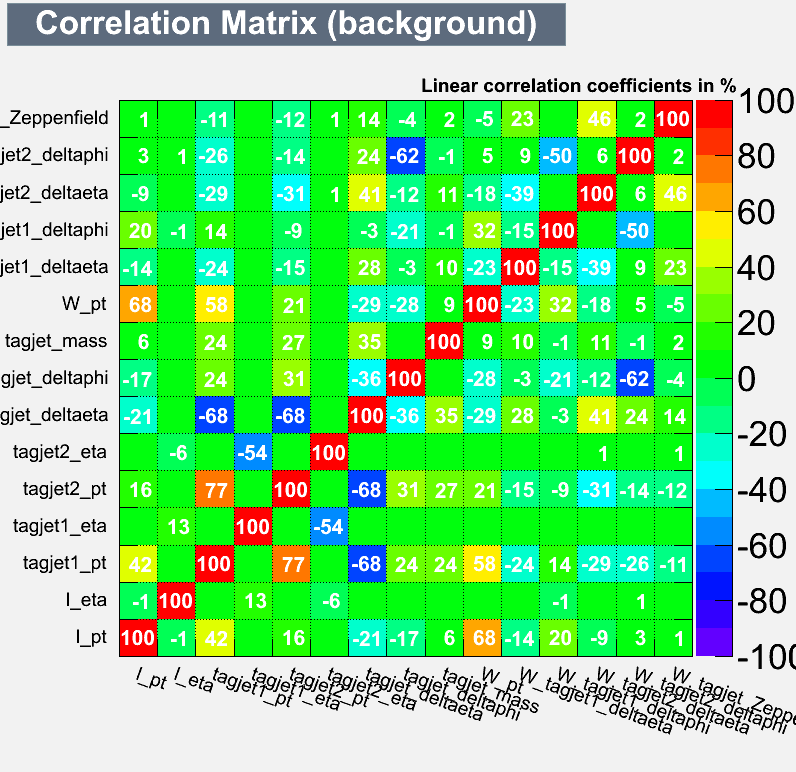
\includegraphics[width=.49\textwidth]{figs/bdtoutput/EWKW2jets_mu_0to100_BDT_traning2_lite_mjj_300root_CorrelationMatrixB.png}
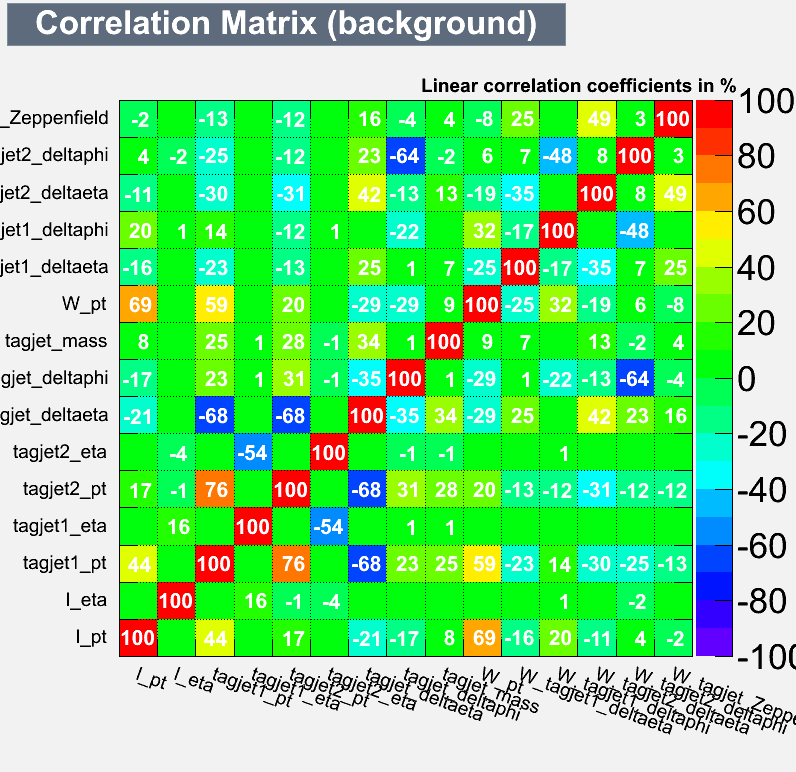
\includegraphics[width=.49\textwidth]{figs/bdtoutput/EWKW2jets_el_0to100_BDT_traning2_lite_mjj_300root_CorrelationMatrixB.png}
}
\caption{Background correlation matrix of the BDT input variables in the muons and electrons events.}
\label{fig:correlation_matrix}
\end{figure}

\begin{figure}[ht]
\centerline{
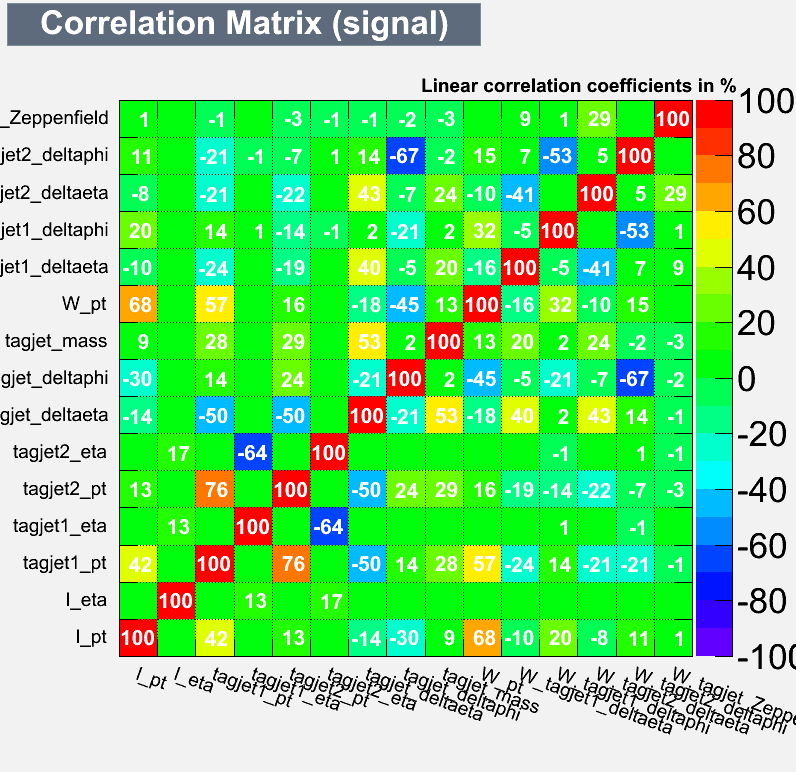
\includegraphics[width=.49\textwidth]{figs/bdtoutput/EWKW2jets_mu_0to100_BDT_traning2_lite_mjj_300root_CorrelationMatrixS.png}
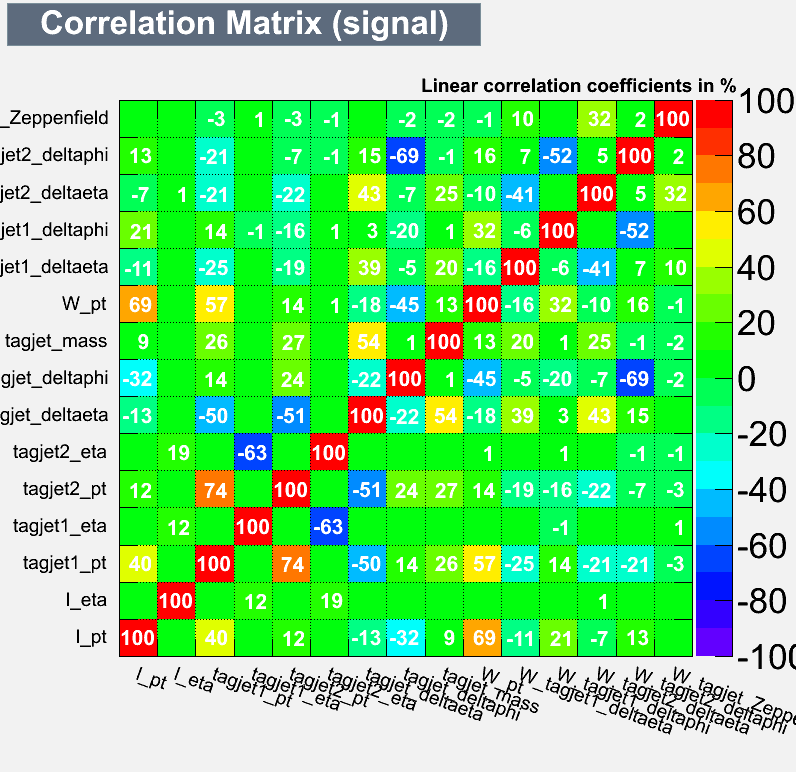
\includegraphics[width=.49\textwidth]{figs/bdtoutput/EWKW2jets_el_0to100_BDT_traning2_lite_mjj_300root_CorrelationMatrixS.png}
}
\caption{Signal correlation matrix of the BDT input variables in the muons and electrons events.}
\label{fig:correlation_matrix}
\end{figure}

\begin{figure}[ht]
\centerline{
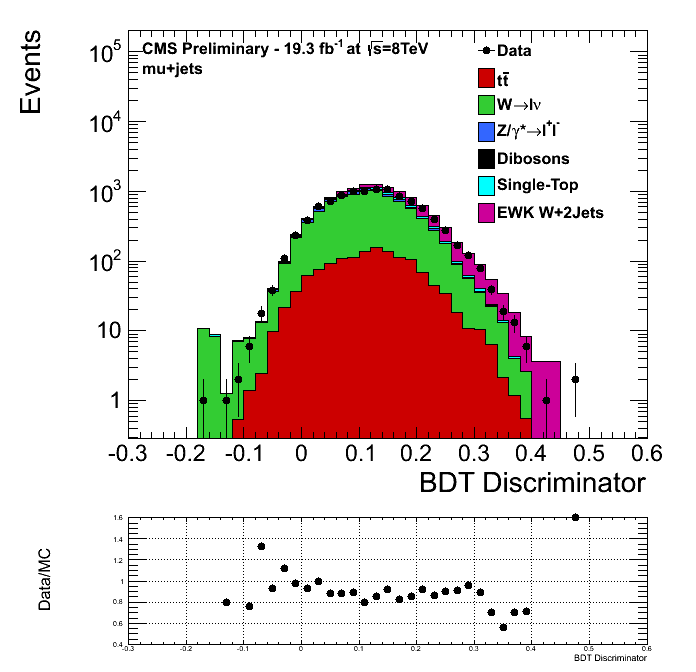
\includegraphics[width=.49\textwidth]{figs/bdtoutput/EWKW2jetsplotmu_mjj1000.png}
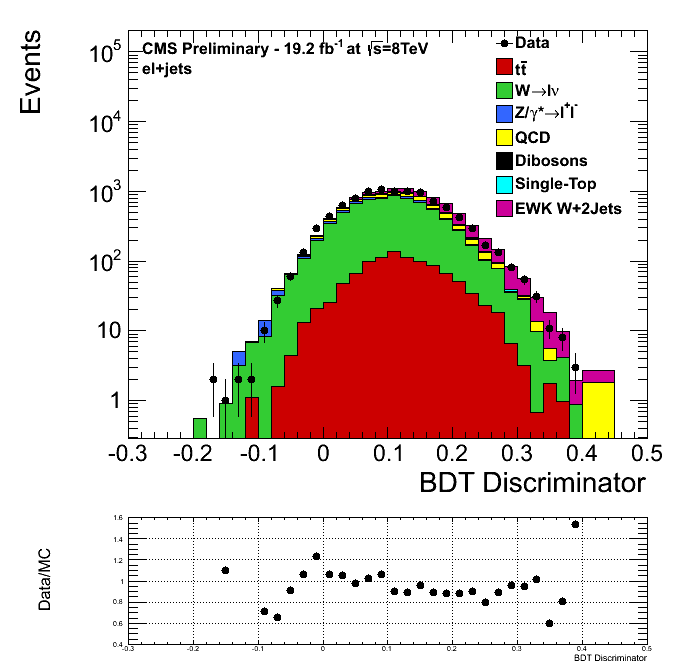
\includegraphics[width=.49\textwidth]{figs/bdtoutput/EWKW2jetsplotelmjj1000.png}
}
\caption{BDT discriminant output in muons (left) and electrons (right) events.}
\label{fig:BDToutputdistribution}
\end{figure}


%\begin{table}[htb]
%\centering
%\begin{tabular}{|c|c|c|}
%\hline
%Channels &  Muons & Electrons \\ \hline
%Wjets scale factor fit result & & \\ \hline
%\end{tabular}
%\caption{Wjets yield scale factor in the reverse BDT output distribution fit}
%\label{tab:bdtfitcontrol}
%\end{table}
%
%\begin{table}[htb]
%\centering
%\begin{tabular}{|c|c|c|}
%\hline
%Channels &  Muons & Electrons \\ \hline
%signal strength fit result & 0.956$\pm$0.121 & \\ \hline
%\end{tabular}
%\caption{EWKW2jets signal strength fit result in the BDT output distribution fit}
%\label{tab:bdtfitresult}
%\end{table}
%We also compare the variables shape in the Appendix~ref{App:shape_compare}.

\clearpage
